\documentclass{beamer}
\usepackage[utf8]{inputenc}
\usepackage{hyperref}
\usepackage{graphicx}
\usepackage{caption}
\usetheme{Madrid}
\usecolortheme{default}


\usepackage{natbib}
\bibliographystyle{abbrvnat}
\setcitestyle{authoryear} %Citation-related commands
% Customizing the citation appearance
\usepackage{xcolor}
\definecolor{darkblue}{RGB}{0,0,139} % Define the dark blue color
\hypersetup{
    colorlinks=true,
    linkcolor=,
    filecolor=,
    urlcolor=,
    citecolor=darkblue % Set the color for citations
}
\usepackage{etoolbox}

% Change citation font size to footnote size
% \makeatletter
% \renewcommand\NAT@open[1]{\textsuperscript{\tiny{#1}}}
% \makeatother

\usepackage{makecell}  




%------------------------------------------------------------
%This block of code defines the information to appear in the
%Title page
\title[Master's Thesis] %optional
{A Study of Text Summarization with Graph Attention Networks}

% \subtitle{Week 8}

\author[Ardestani, Reza] % (optional)
{~Ardestani, MohammadReza\inst{1} }

\institute[] % (optional)
{
  \inst{1}%
  Department of Computer Science\\
  University of Lethbridge\\
  ardestani@uleth.ca
}

\date[Aug 2024] % (optional)
{Aug 19, 2024}

\logo{
\includegraphics[height=0.5cm]{uleth_logo.png}}

%End of title page configuration block
%------------------------------------------------------------



%------------------------------------------------------------
%The next block of commands puts the table of contents at the 
%beginning of each section and highlights the current section:

\AtBeginSection[]
{
  \begin{frame}
    \frametitle{Table of Contents}
    \tableofcontents[currentsection]
  \end{frame}
}
%------------------------------------------------------------


\begin{document}

%The next statement creates the title page.
\frame{\titlepage}




%---------------------------------------------------------
%This block of code is for the table of contents after
%the title page
\begin{frame}
\frametitle{Acknowledgment}
\textcolor{red}{\textbf{Supervisor:}} I extend my deepest gratitude to Dr. \textbf{Yllias Chali}, whose continuous support and guidance have been the cornerstone of my journey.\vspace{5px}

\textcolor{red}{\textcolor{red}{\textbf{Committee:}}} My sincere appreciation goes to the committee members, Dr. \textbf{John Anvik} and Dr. \textbf{John Sheriff}, for their constructive feedback throughout several Progress Standing meetings.\vspace{5px}

\textcolor{red}{\textbf{Chair:}} I would like to express my gratitude to Dr. \textbf{Wendy Osborn}, for her unwavering support and her guidance on procedures.\vspace{5px}

\textcolor{red}{\textbf{University of Lethbridge, Alberta Innovates, NSERC:}} I'm immensely grateful for their generous support, allowing me to focus on my research.\vspace{5px}

\textcolor{red}{\textbf{Compute Canada:}} Without the sponsorship of my supervisor for using the well-maintained High Performance Clusters of Compute Canada, conducting this research was not possible.

\textcolor{red}{\textbf{Internship Students:}} I had a pleasure to work with Taha Abbass and Riya Saxena whose contribution to the dataset processing were valuable.





\end{frame}
%---------------------------------------------------------


%---------------------------------------------------------
%This block of code is for the table of contents after
%the title page
\begin{frame}
\frametitle{Table of Contents}
\tableofcontents
\end{frame}
%---------------------------------------------------------


\section{Overview}

%---------------------------------------------------------
\begin{frame}
  \frametitle{Overview}

  \begin{minipage}[t][0.6\textheight][t]{\textwidth}
    \centering
    \begin{minipage}{0.3\textwidth}
      \centering
        \begin{figure}[ht]
            \centering
            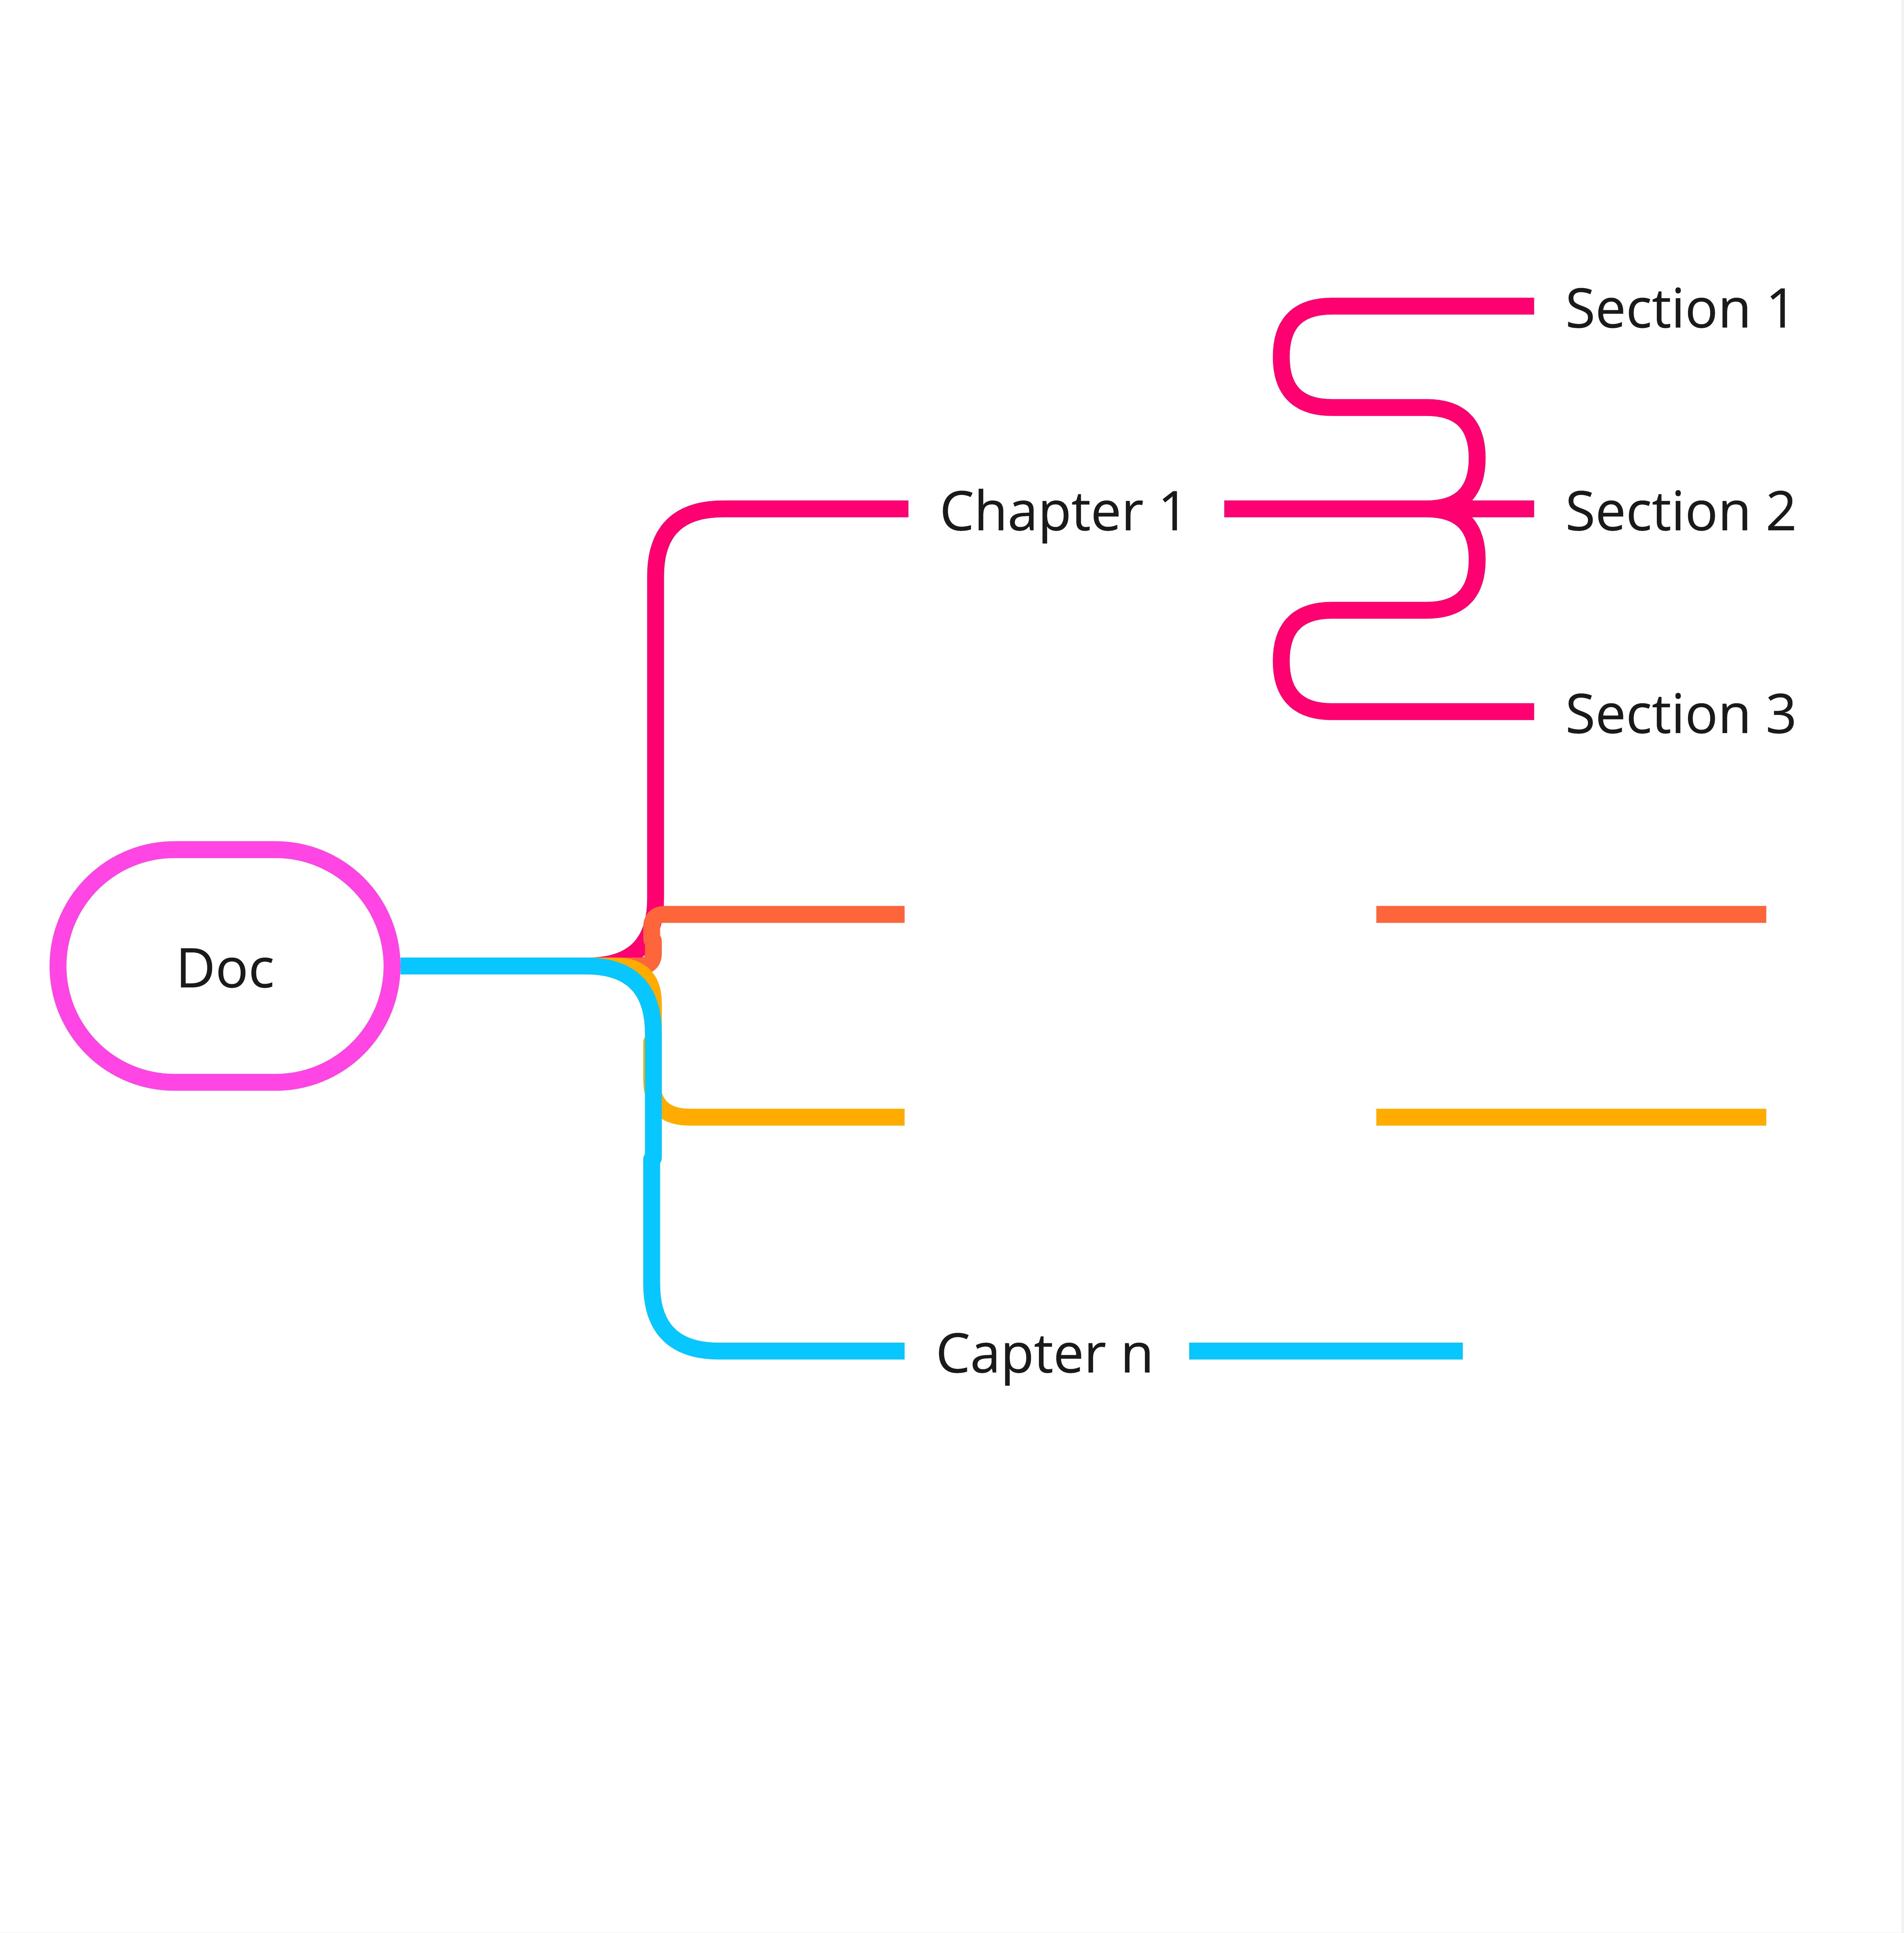
\includegraphics[width=\textwidth]{imgs/chapter_section_.jpg}
            \caption*{Chapter-Section graph}
        \end{figure}
    \end{minipage}%
    % \pause
    \hfill
    \begin{minipage}{0.3\textwidth}
      \centering
        \begin{figure}[ht]
            \centering
            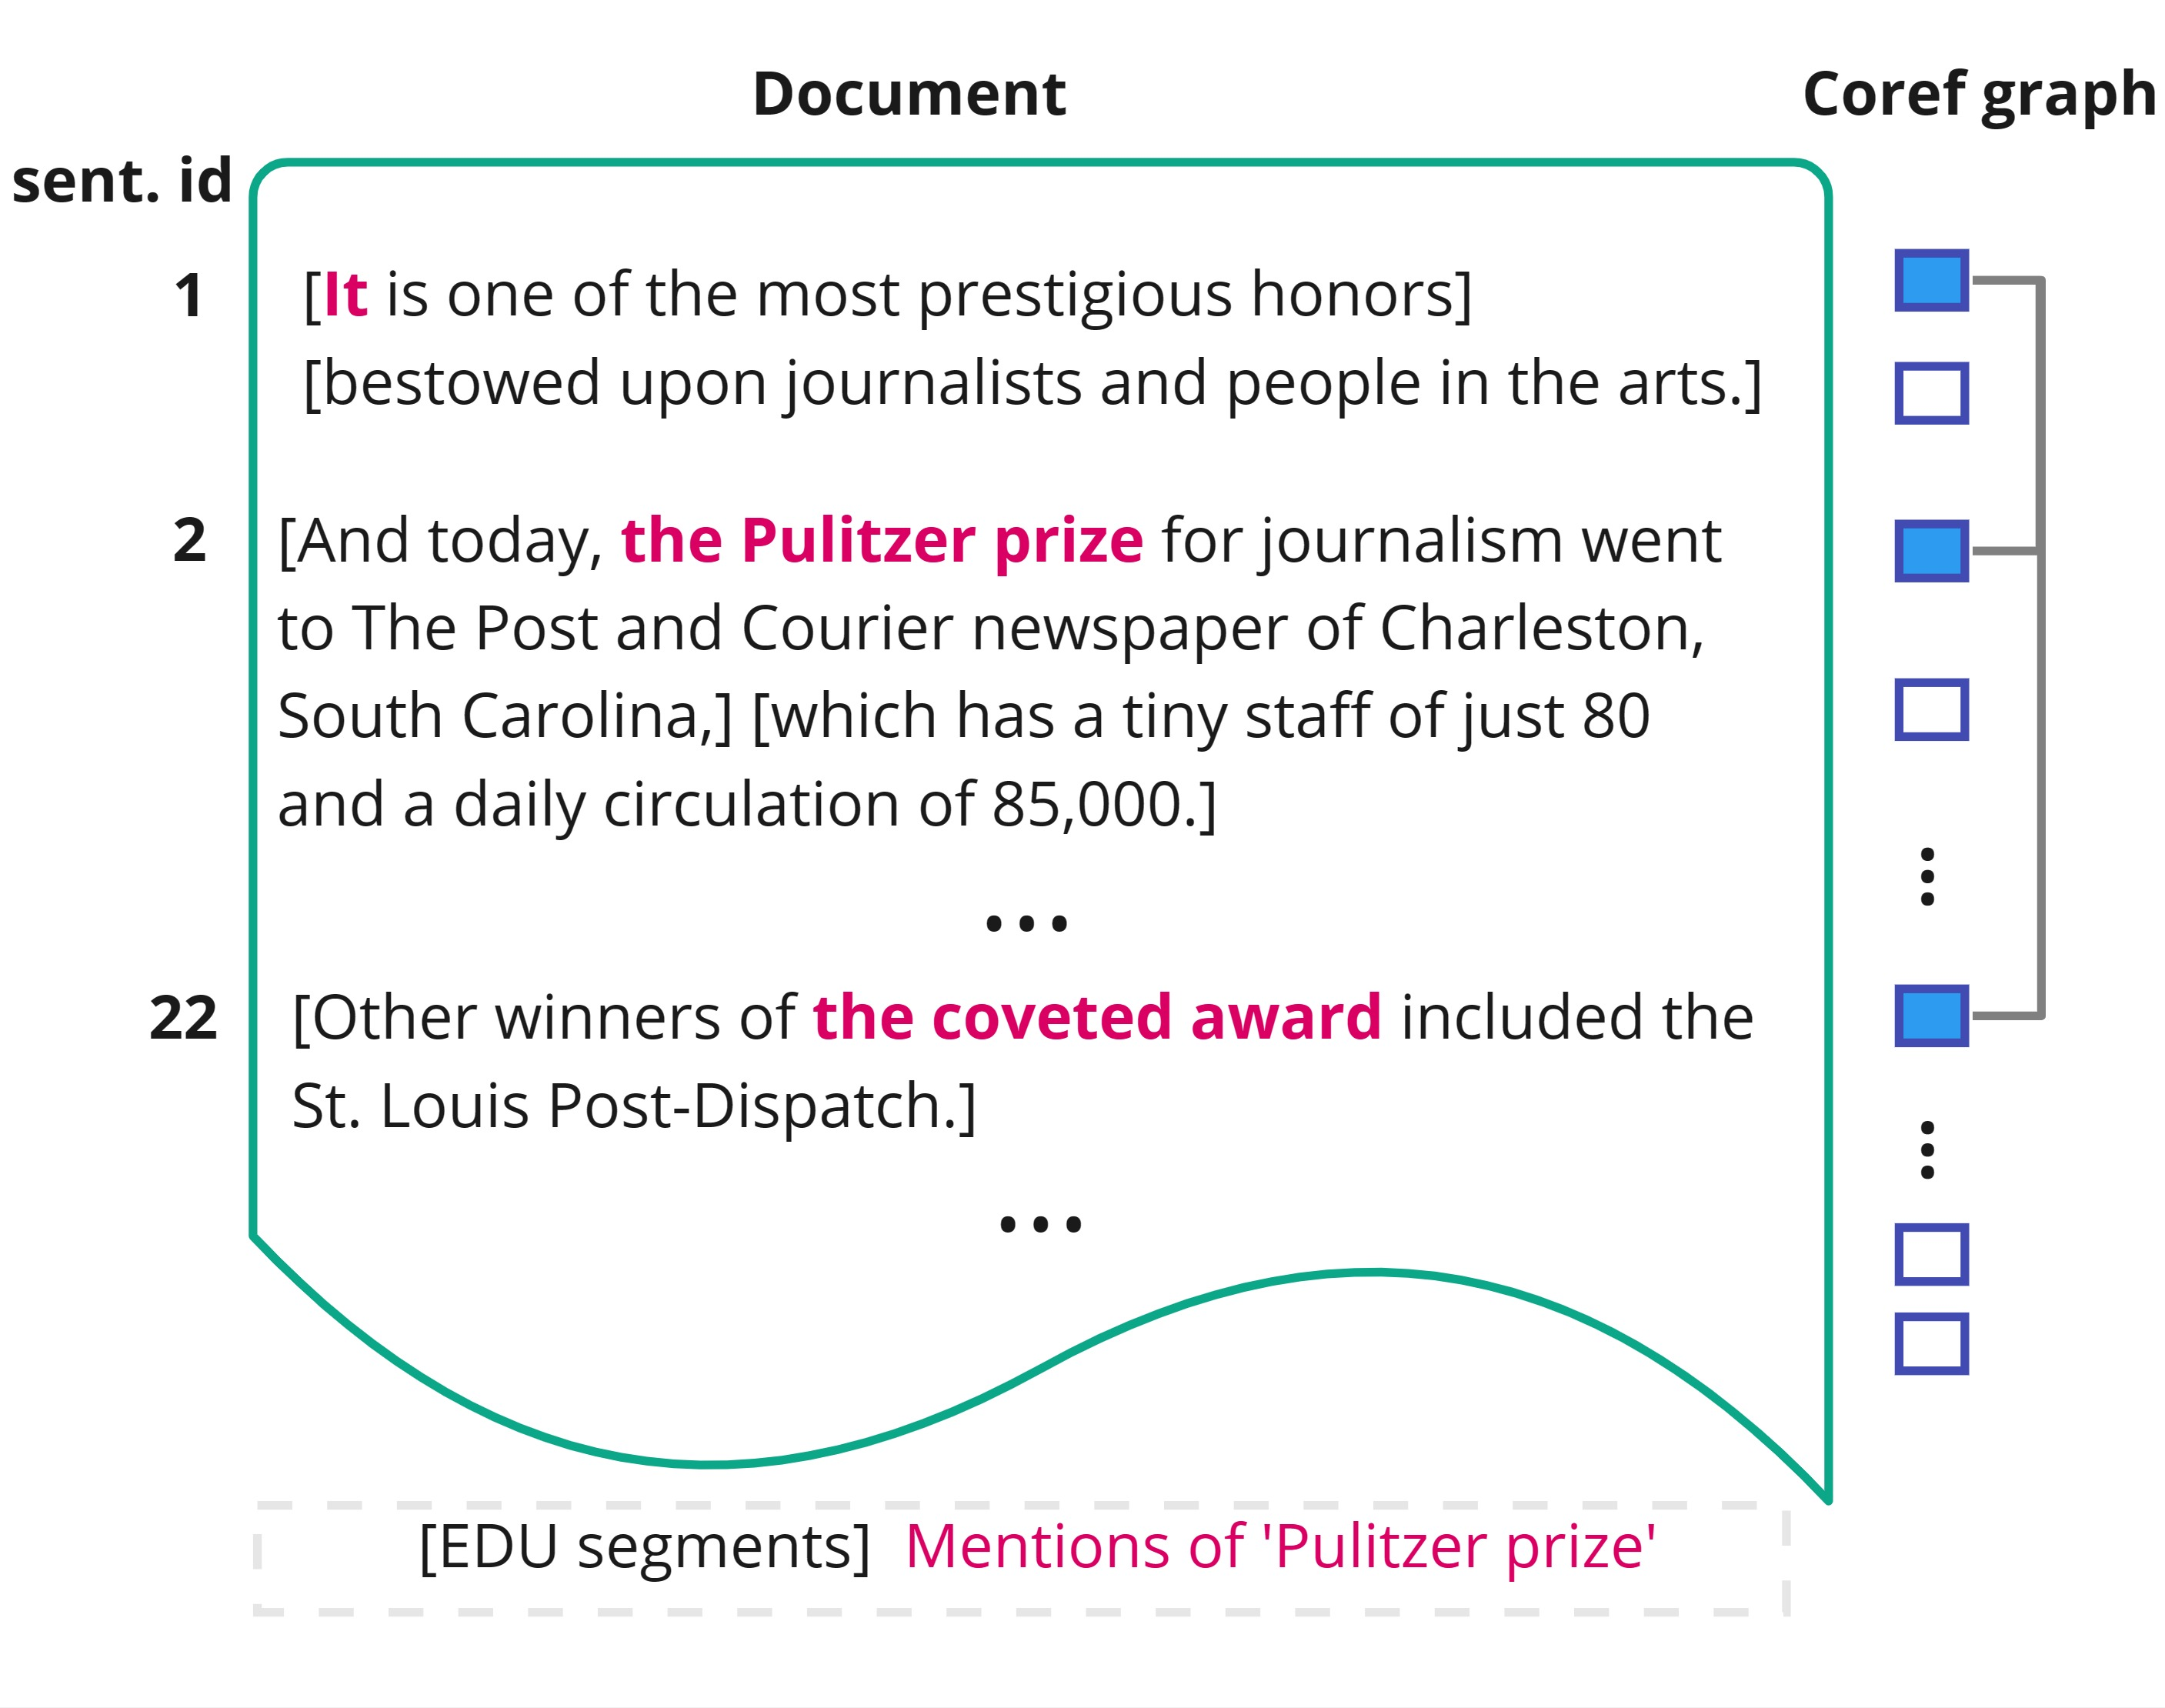
\includegraphics[width=\textwidth]{imgs/co-reference-example.jpg}
            \caption*{Coref graph}
            {\tiny adopted from \citep{DiscoBERT}}
        \end{figure}
    \end{minipage}%
    \hfill
    \begin{minipage}{0.3\textwidth}
      \centering
        \begin{figure}[ht]
            \centering
            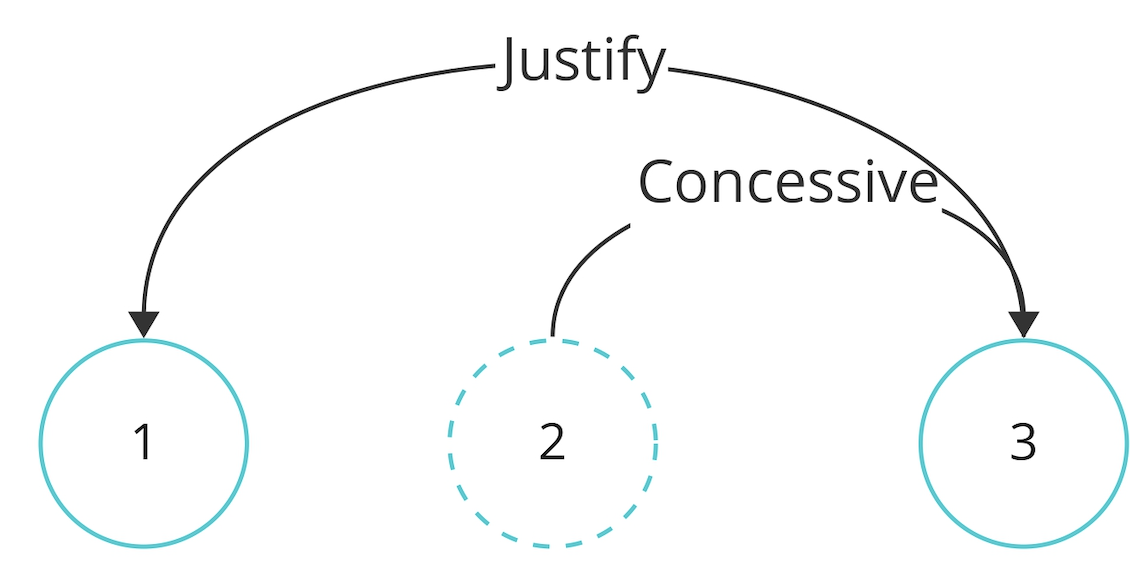
\includegraphics[width=\textwidth]{imgs/rst_graph.png}
            \caption*{RST graph}
            {\tiny adopted \citep{rst1988}}
        \end{figure}
    \end{minipage}
    % \pause
  \end{minipage}
 

  \begin{minipage}[t][0.4\textheight][t]{\textwidth}
    \begin{itemize}
      \item We naturally form a chapter-section graph of a document in our mind to understand that better.      % \pause
      \item We used two similar graphs which facilitate summarization; RST {\tiny \citep{rst1988}} \& Coref {\tiny \citep{coreference-review}}
    \end{itemize}
  \end{minipage}

\end{frame}

%---------------------------------------------------------





\section{Introduction}


%---------------------------------------------------------
%Highlighting text
\begin{frame}
\frametitle{Introduction}

\begin{block}{Summarization; an unsolved problem}
Unlike Machine Translation {\tiny \citep{Popel2020}}, Automatic Text Summarization is remained far from achieving human-level performance {\tiny \citep{summarizationSurvey-waffa-el-kassas}}.
\end{block}
% \pause

\begin{alertblock}{Transformer; a prevailing yet problematic architecture}
Despite their success in machine translation, transformers struggle with more complex tasks like Dialogue Management and Text Summarization.
\end{alertblock}
% \pause

\begin{exampleblock}{Graph; a guiding structure}
Recent findings indicate that graphs can enhance the performance in T2T generation tasks {\tiny \citep{GNNBook-ch21-liu}}.
\end{exampleblock}

\end{frame}
%---------------------------------------------------------


\section{Related Works}

%---------------------------------------------------------
%Changing visivility of the text
\begin{frame}
\frametitle{Top Three Related Works}
% \begin{itemize}
%     \item DiscoBERT, a recent \textbf{extractive} approach which segments documents into smaller units, known as EDU, then leverages two graph structures for extracting important parts as the final summary.\vspace{10px}
    
%     \item BART, a recent \textbf{abstractive} approach which trained using a denoising autoencoder approach and combines the power of BERT and GPT to handle a variety of text generation and comprehension tasks. \vspace{10px}
    
%     \item BERTEXTABS, a recent \textbf{hybrid} approach which uses a fine-tuned BERT for selecting the important part, then pass it to a trained transformers to generated the final summaries.
% \end{itemize}

\begin{table}[h!]
    \footnotesize
    \centering
    \begin{tabular}{p{2cm}p{1cm}p{8cm}}
        \hline
        \textbf{Model} & \textbf{Type} & \textbf{\:\:\:\:Distinctive Features} \\ \hline \\
        DiscoBERT {\tiny \citep{DiscoBERT}} & Extractive & \vspace{-\baselineskip} % Adjust space above itemize
        \begin{itemize}
            \setlength{\itemsep}{0pt}%
            \setlength{\topsep}{0pt}%
            \item Segments documents to smaller units (EDUs)
            \item Leverages two graph structures for extraction
        \end{itemize} \\ 
        BART \: \: \: \: \:{\tiny \citep{bart}} & Abstractive & \vspace{-\baselineskip} % Adjust space above itemize
        \begin{itemize}
            \item Trained using a denoising autoencoder approach
            \item Combines the power of BERT and GPT
            \item Handles a variety of text generation and comprehension tasks
        \end{itemize} \\
        BERTEXTABS {\tiny \citep{BertSum}} & Hybrid & \vspace{-\baselineskip} % Adjust space above itemize
        \begin{itemize}
            \item Fine-tuned BERT for selecting important parts, then a trained transformer to generate the final summaries
        \end{itemize} \\ \hline
    \end{tabular}
    % \caption{Comparison of Different Summarization Models}
    % \label{tab:summarization_models}
\end{table}

% We mainly adopted these works \& introduced our novelty to enhance performance.


 

\end{frame}




%---------------------------------------------------------



\section{Dataset Preparation}

%---------------------------------------------------------
%Changing visivility of the text
\begin{frame}
\frametitle{Dataset Prepration Pipeline}

   \begin{minipage}[t][0.5\textheight][t]{\textwidth}
      \centering
      \includegraphics[scale=0.05]{{imgs/thesie_pipeline_blue.jpg}} 
  \end{minipage}

  \vfill

  \begin{minipage}[t][0.3\textheight][t]{\textwidth}
    \begin{itemize}
      \item We batched XSum {\tiny \cite{xsum}} documents into 10K-size files and then distributed the process on eight servers to reduce the process time from 29 days to roughly 3 days.
    \end{itemize}
  \end{minipage}
  
% \begin{center}
% \includegraphics[scale=.056]{imgs/thesie_pipeline_blue.jpg}
% \end{center}

\end{frame}

%---------------------------------------------------------


%---------------------------------------------------------
%Changing visivility of the text
\begin{frame}
\frametitle{Stats of the Generated Dataset}

\begin{center}
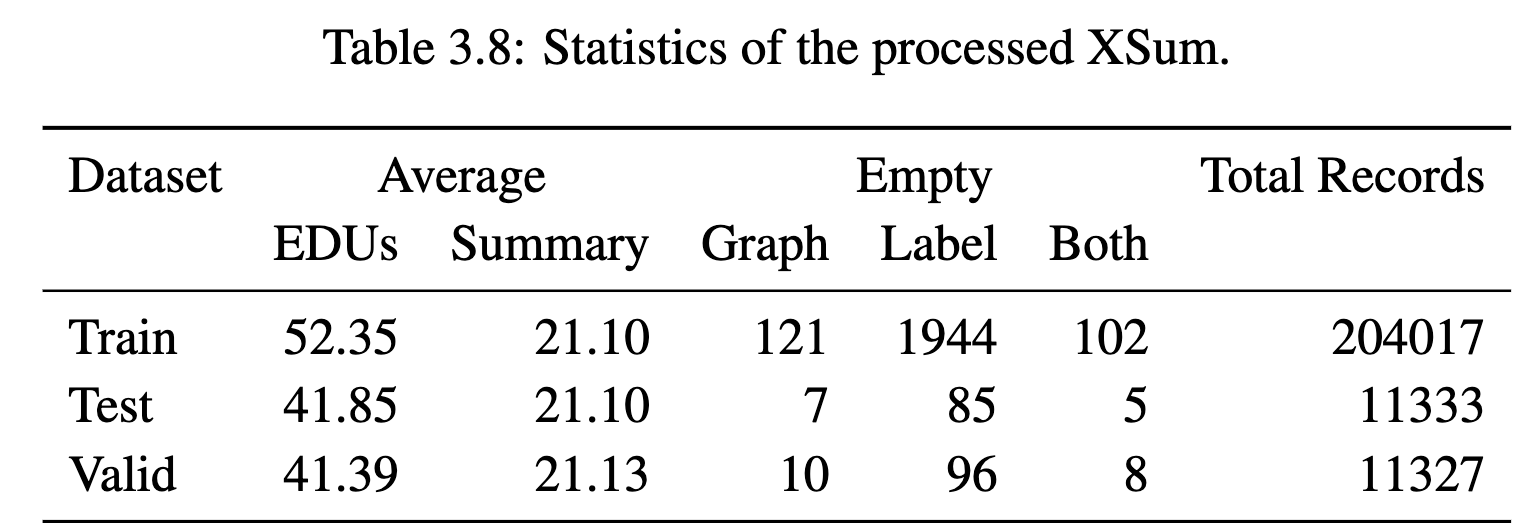
\includegraphics[scale=.4]{imgs/stats_of_generated_xsum.png}
\end{center}
  \begin{minipage}[t][0.3\textheight][t]{\textwidth}
    \begin{itemize}
      \item Unlike CNN/DM, XSum summaries are short, averaging 21 words.
      \item Unlike CNN/DM, the summaries are extremely paraphrased.
      \item We undertook a costly dataset generation for two main reasons:
      \begin{itemize}
          \item Bias reduction 
          \item Robustness
      \end{itemize}
    \end{itemize}
  \end{minipage}

\end{frame}

%---------------------------------------------------------

\section{Proposed Model}


% %---------------------------------------------------------
% \begin{frame}
% \frametitle{Generation \& Fine-tuning Pipeline}

% % \begin{center}
% %     \includegraphics[scale=0.3]{w8_4.png}
% % \end{center}

% \tiny{[Photo from \href{https://www.coursera.org/learn/nlp-sequence-models}{nlp-sequence-models}]}


% \end{frame}
% %---------------------------------------------------------

%---------------------------------------------------------
\begin{frame}
\frametitle{Proposed Model Architecture}

\begin{figure}[ht]
    \centering
    \begin{minipage}{0.6\textwidth}
            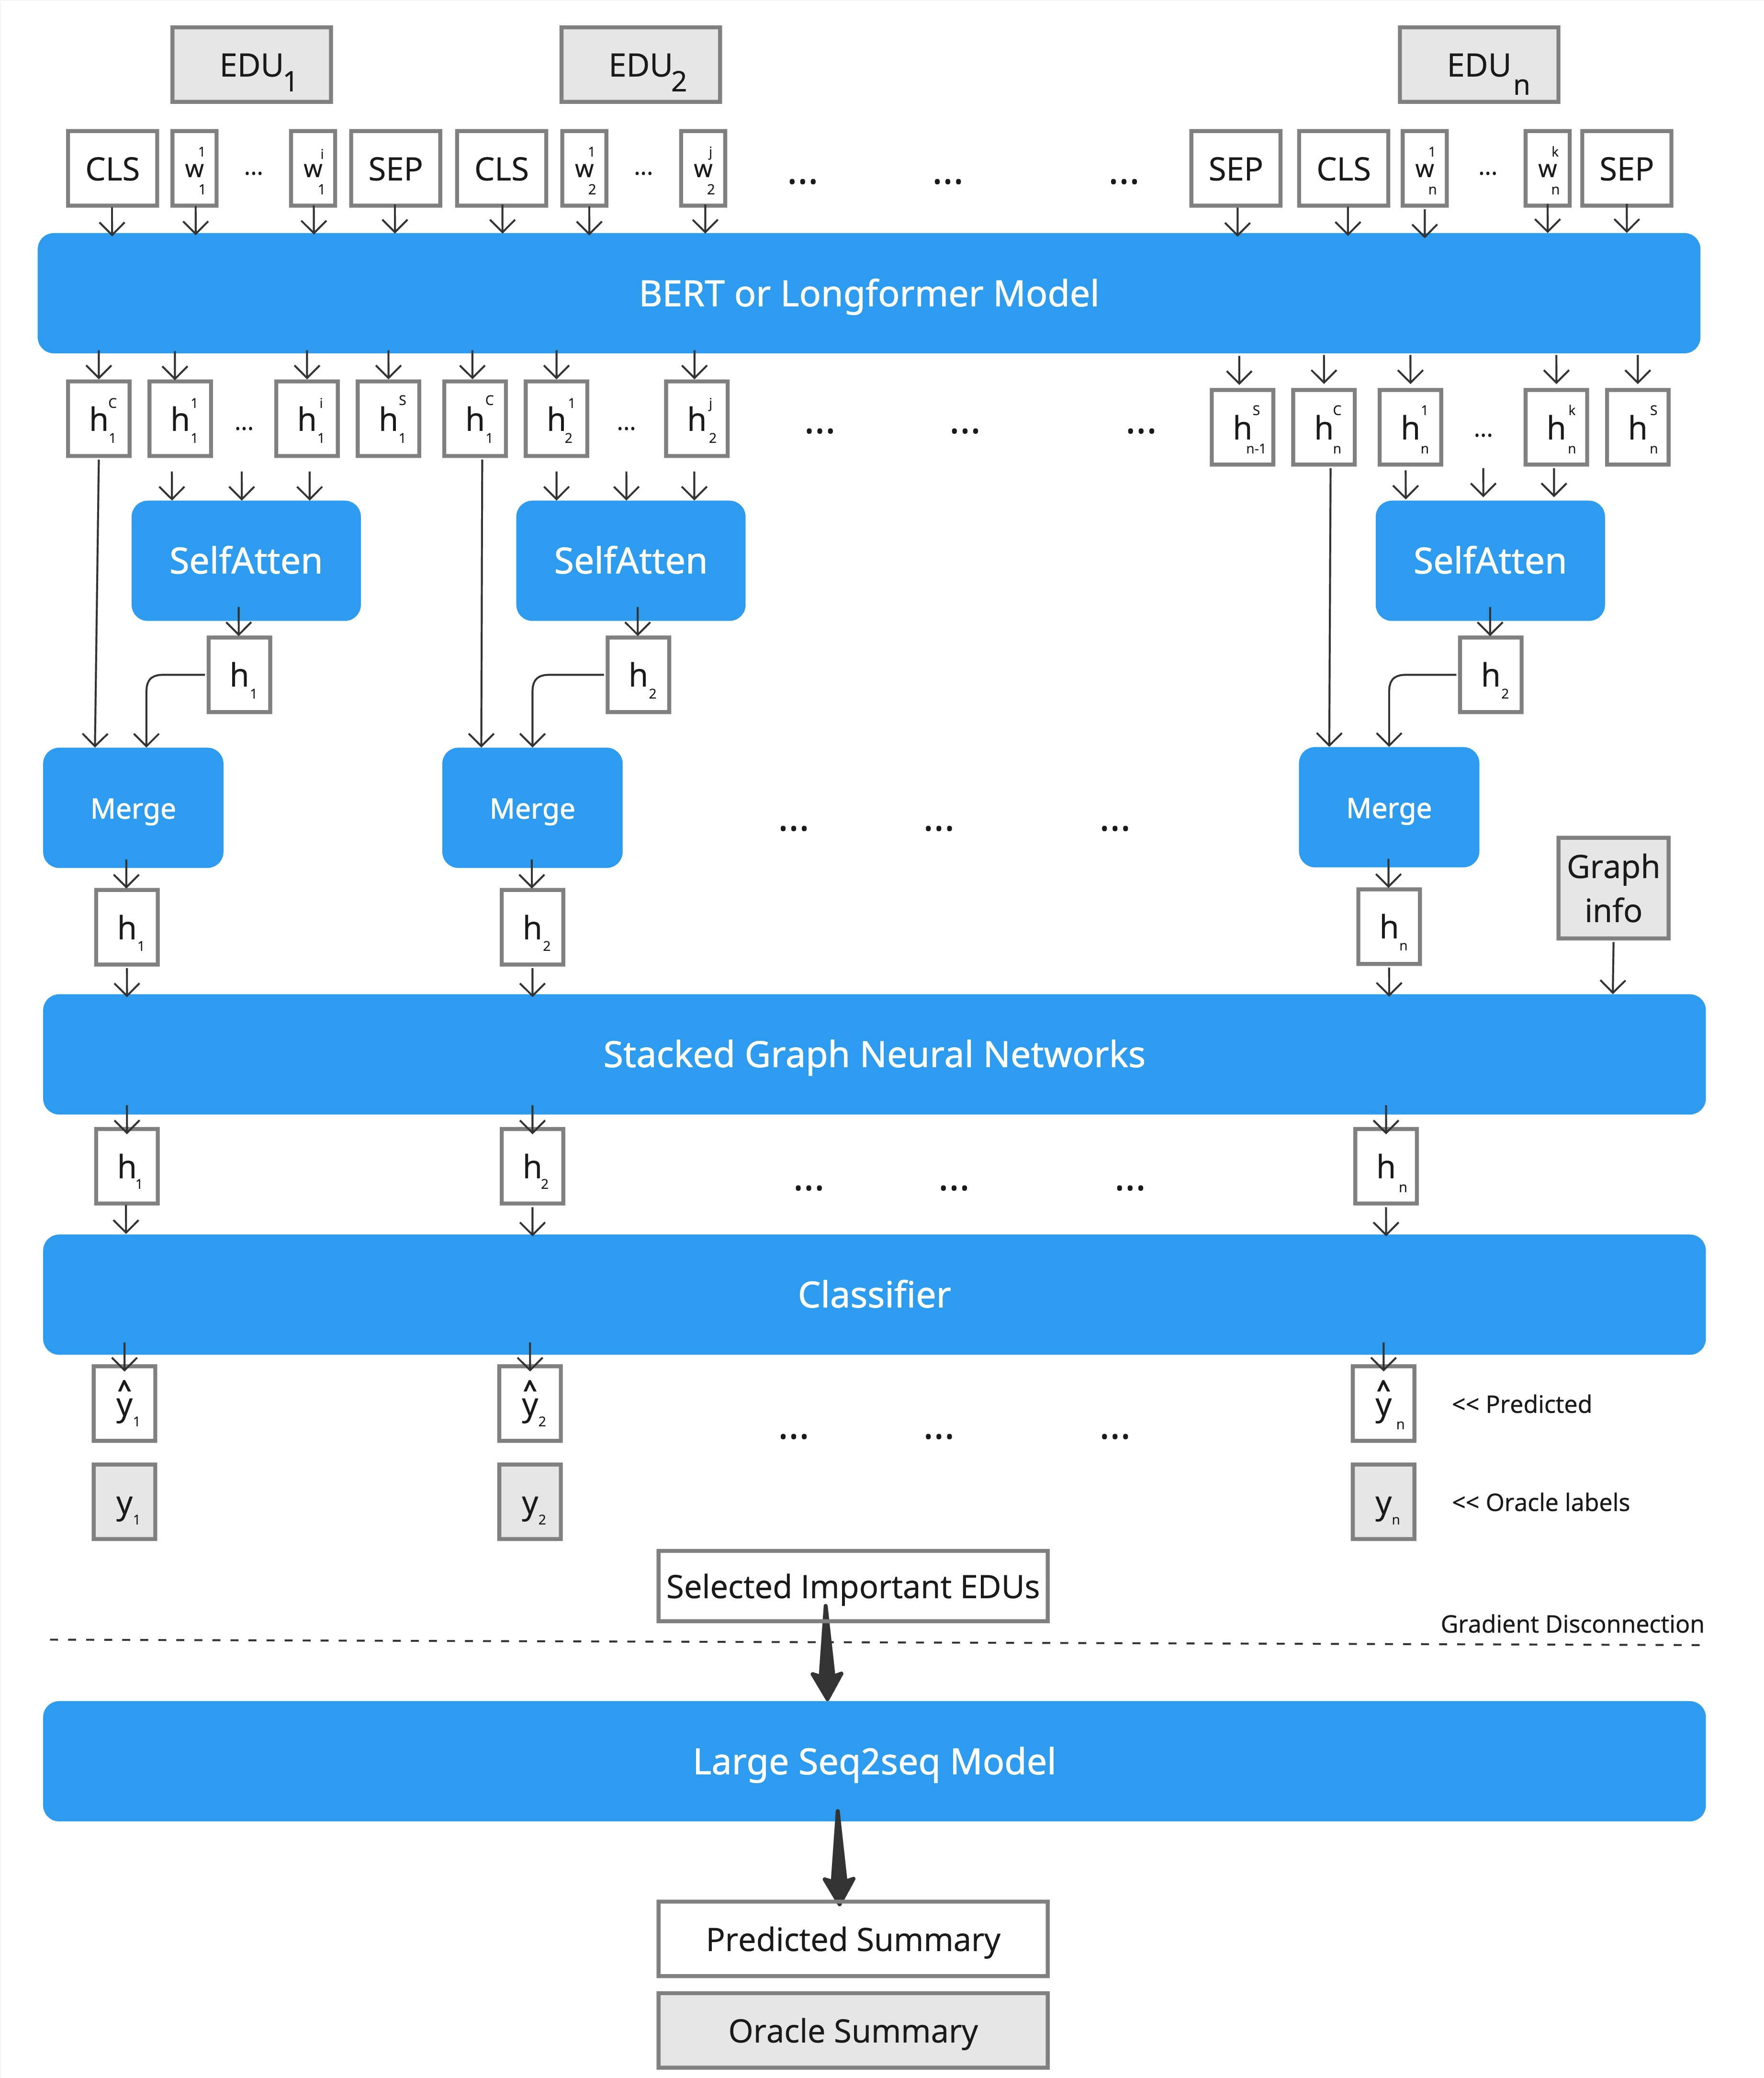
\includegraphics[scale=.05]{imgs/MyModelOverview.jpg}
            \end{minipage}\hfill
    \begin{minipage}{0.4\textwidth}
    \footnotesize
     Our design \& fine-tuning highlights:\\\\
     \textbullet\: Cached tokenized inputs, a repetitive process for all epochs in all experiments, resulted in reduced RAM usage \& runtime\\
     \textbullet\: Vectorized operations for faster matrix multiplication \\
     \textbullet\: Utilized penalty to handle class imbalance \\
    \textbullet\: Leveraged various ML methods to improve the selection F1 score \\
    \textbullet\: Parallelized the fine-tuning to reduce runtime by 75\% \\

    These allowed us to efficiently conduct over 36 main experiments and 500 hyper-parameter searches.

     
            
        % SelfAttentive {\tiny \citep{DiscoBERT}} layer is formulated as:
        % \begin{equation}
        % \label{eq1}
        % H = \text{ReLU}(XW_1 + b_1)
        % \end{equation}
        % \begin{equation}
        % \label{eq2}
        % A = HW_2 + b_2
        % \end{equation}
        % \begin{equation}
        % \label{eq3}
        % \alpha = \text{softmax}(A) = \frac{e^{A_i}}{\sum_{j=1}^{n}e^{A_j}}
        % \end{equation}
        % \begin{equation}
        % \label{eq4}
        % S = \sum_{i=1}^{n}\alpha_i X_i
        % \end{equation}
    \end{minipage}
\end{figure}


\end{frame}
%---------------------------------------------------------


%---------------------------------------------------------
\begin{frame}
\frametitle{GNN}

   \begin{minipage}[t][0.3\textheight][t]{\textwidth}
      \centering
      
\includegraphics[width=\textwidth]{{imgs/fig29.jpg}} 
  \end{minipage}

Graph learning includes two main operations {\tiny \citep{Hamilton-William-graphs}}:
  \begin{minipage}[t][0.7\textheight][t]{\textwidth}
  \vspace{-\baselineskip}
\begin{align}
    m^{(k)}_{N(u)} &= \text{AGGREGATE}^{(k)} \left(\{h_v^{(k)}, \forall v \in N(u)\}\right)\\
    h_u^{(k+1)} &= \text{UPDATE}^{(k)}\left(h_u^{(k)}, m^{(k)}_{N(u)}\right)
\end{align}
\newline

\footnotesize
Besides GAT, we also experimented with different GNN architectures, namely, GCN.

\end{minipage}


\end{frame}
%---------------------------------------------------------


%---------------------------------------------------------
\begin{frame}
\frametitle{MLP Variation \& Input}


\begin{figure}[ht]
    \centering
    \begin{minipage}{0.5\textwidth}
            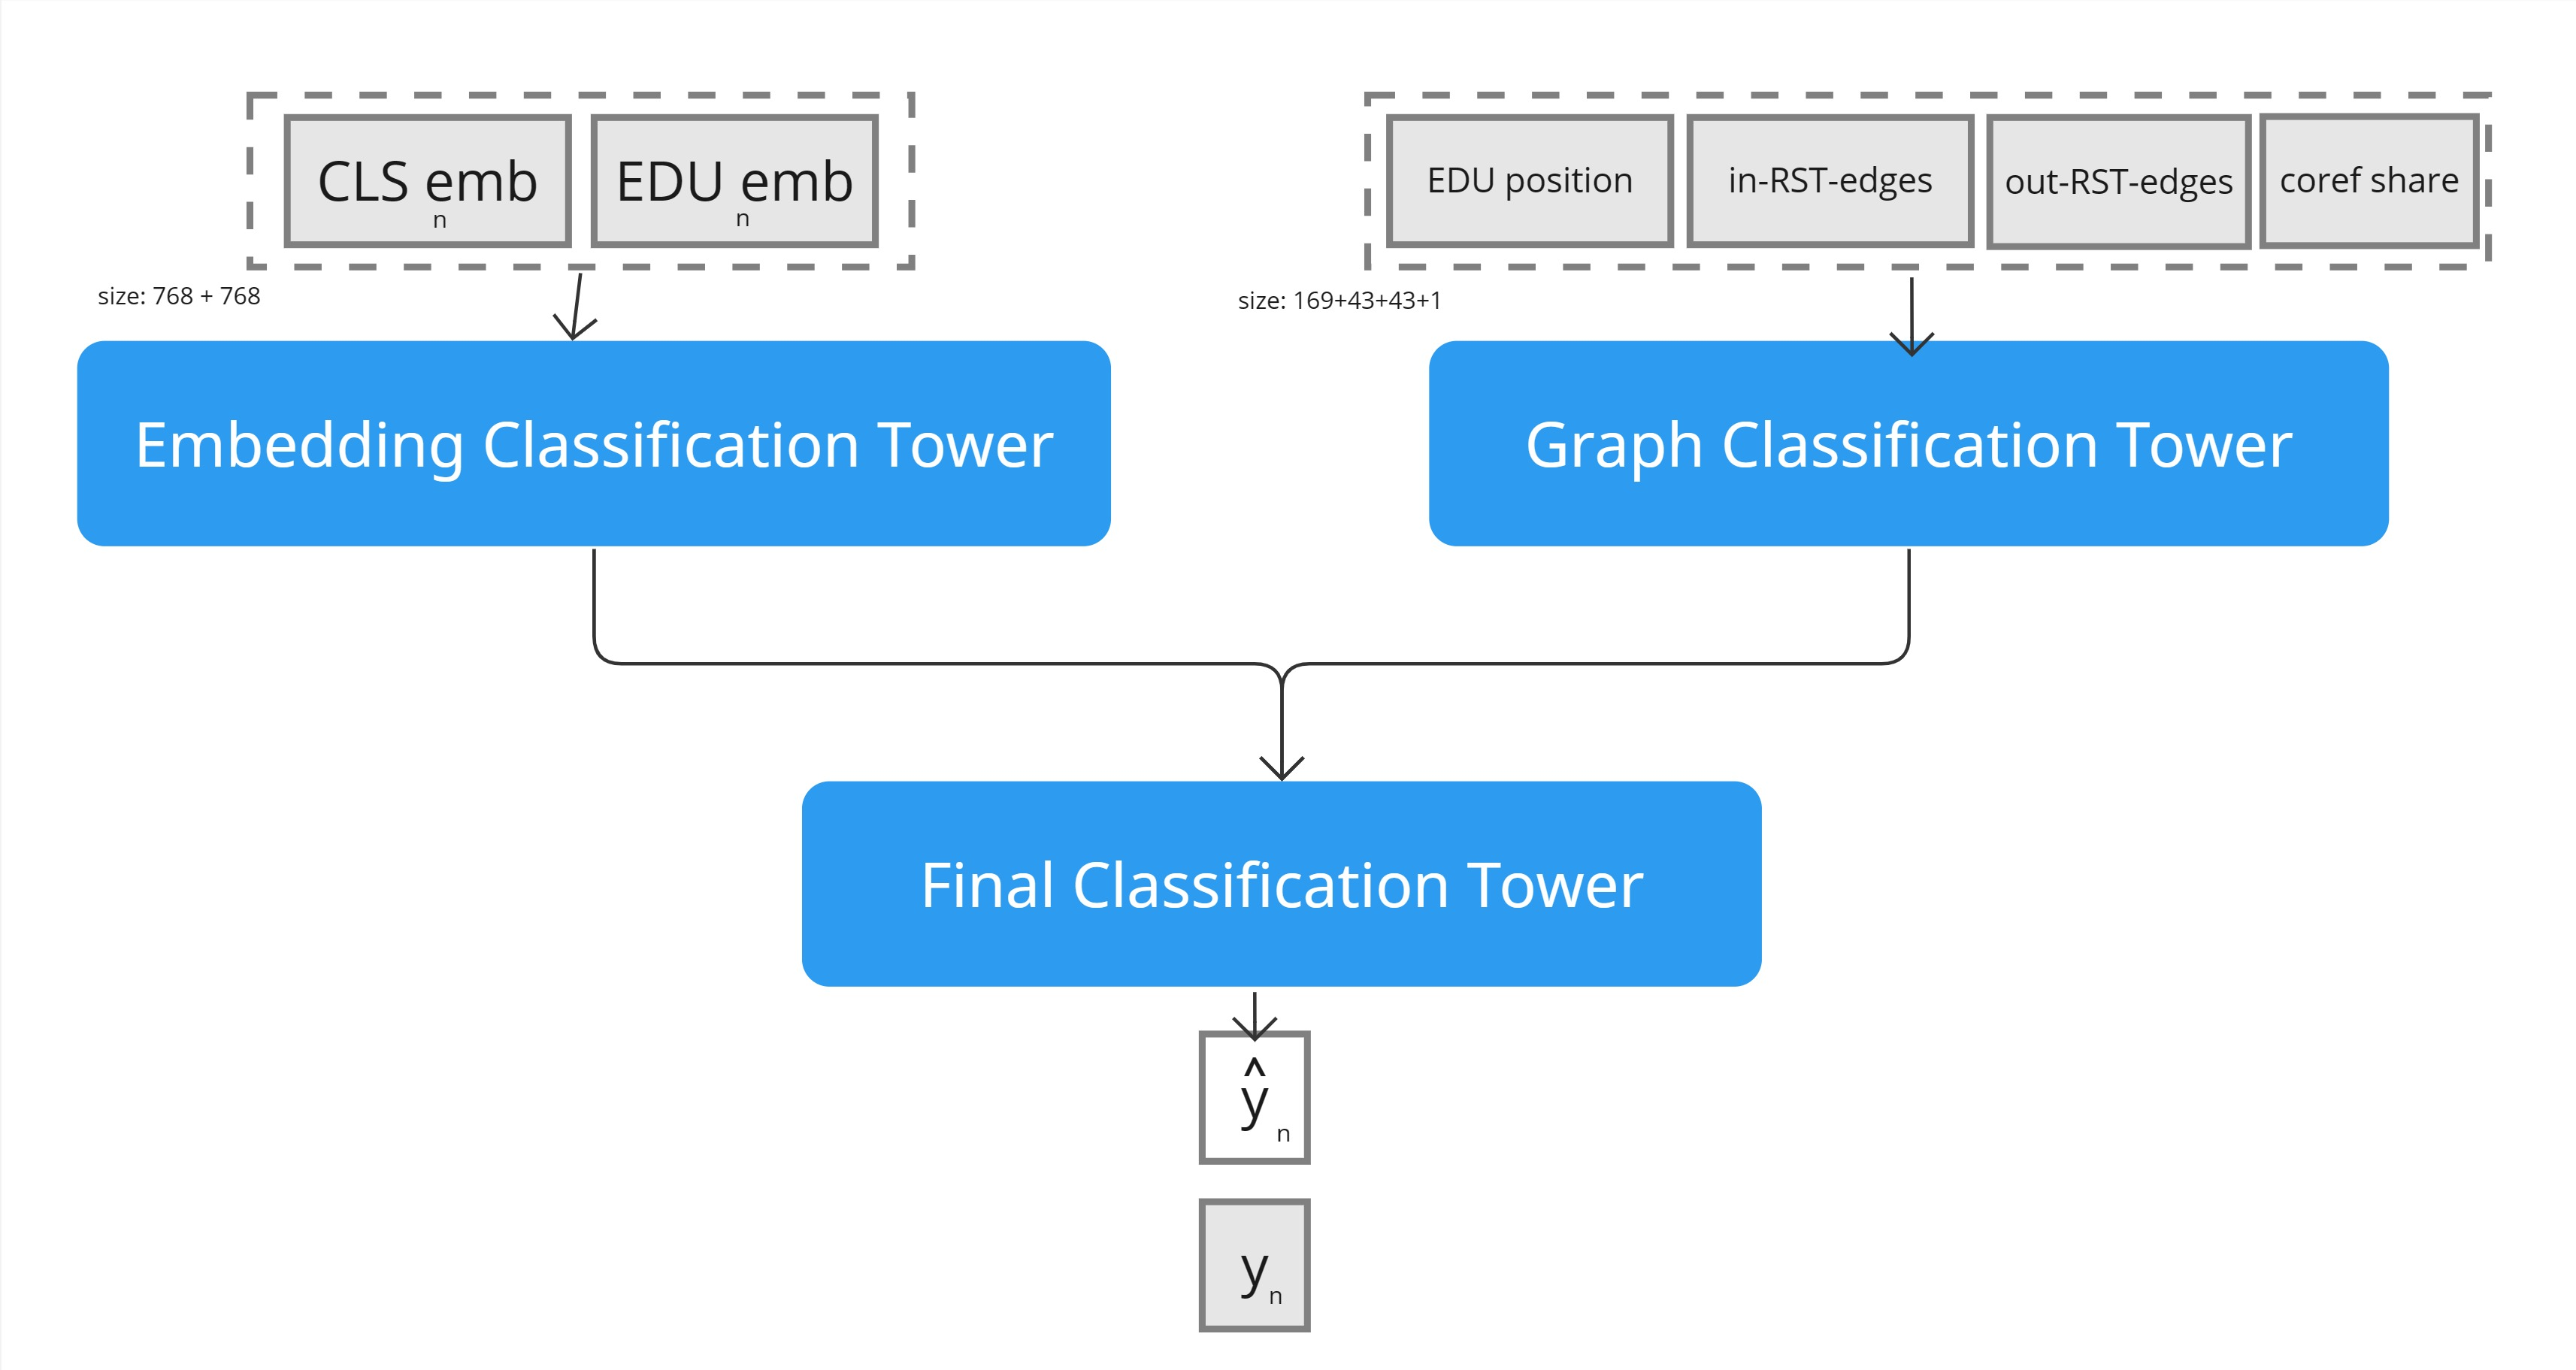
\includegraphics[scale=.05]{imgs/novel_approach.jpg}
            \end{minipage}\hfill
    \begin{minipage}{0.5\textwidth}
    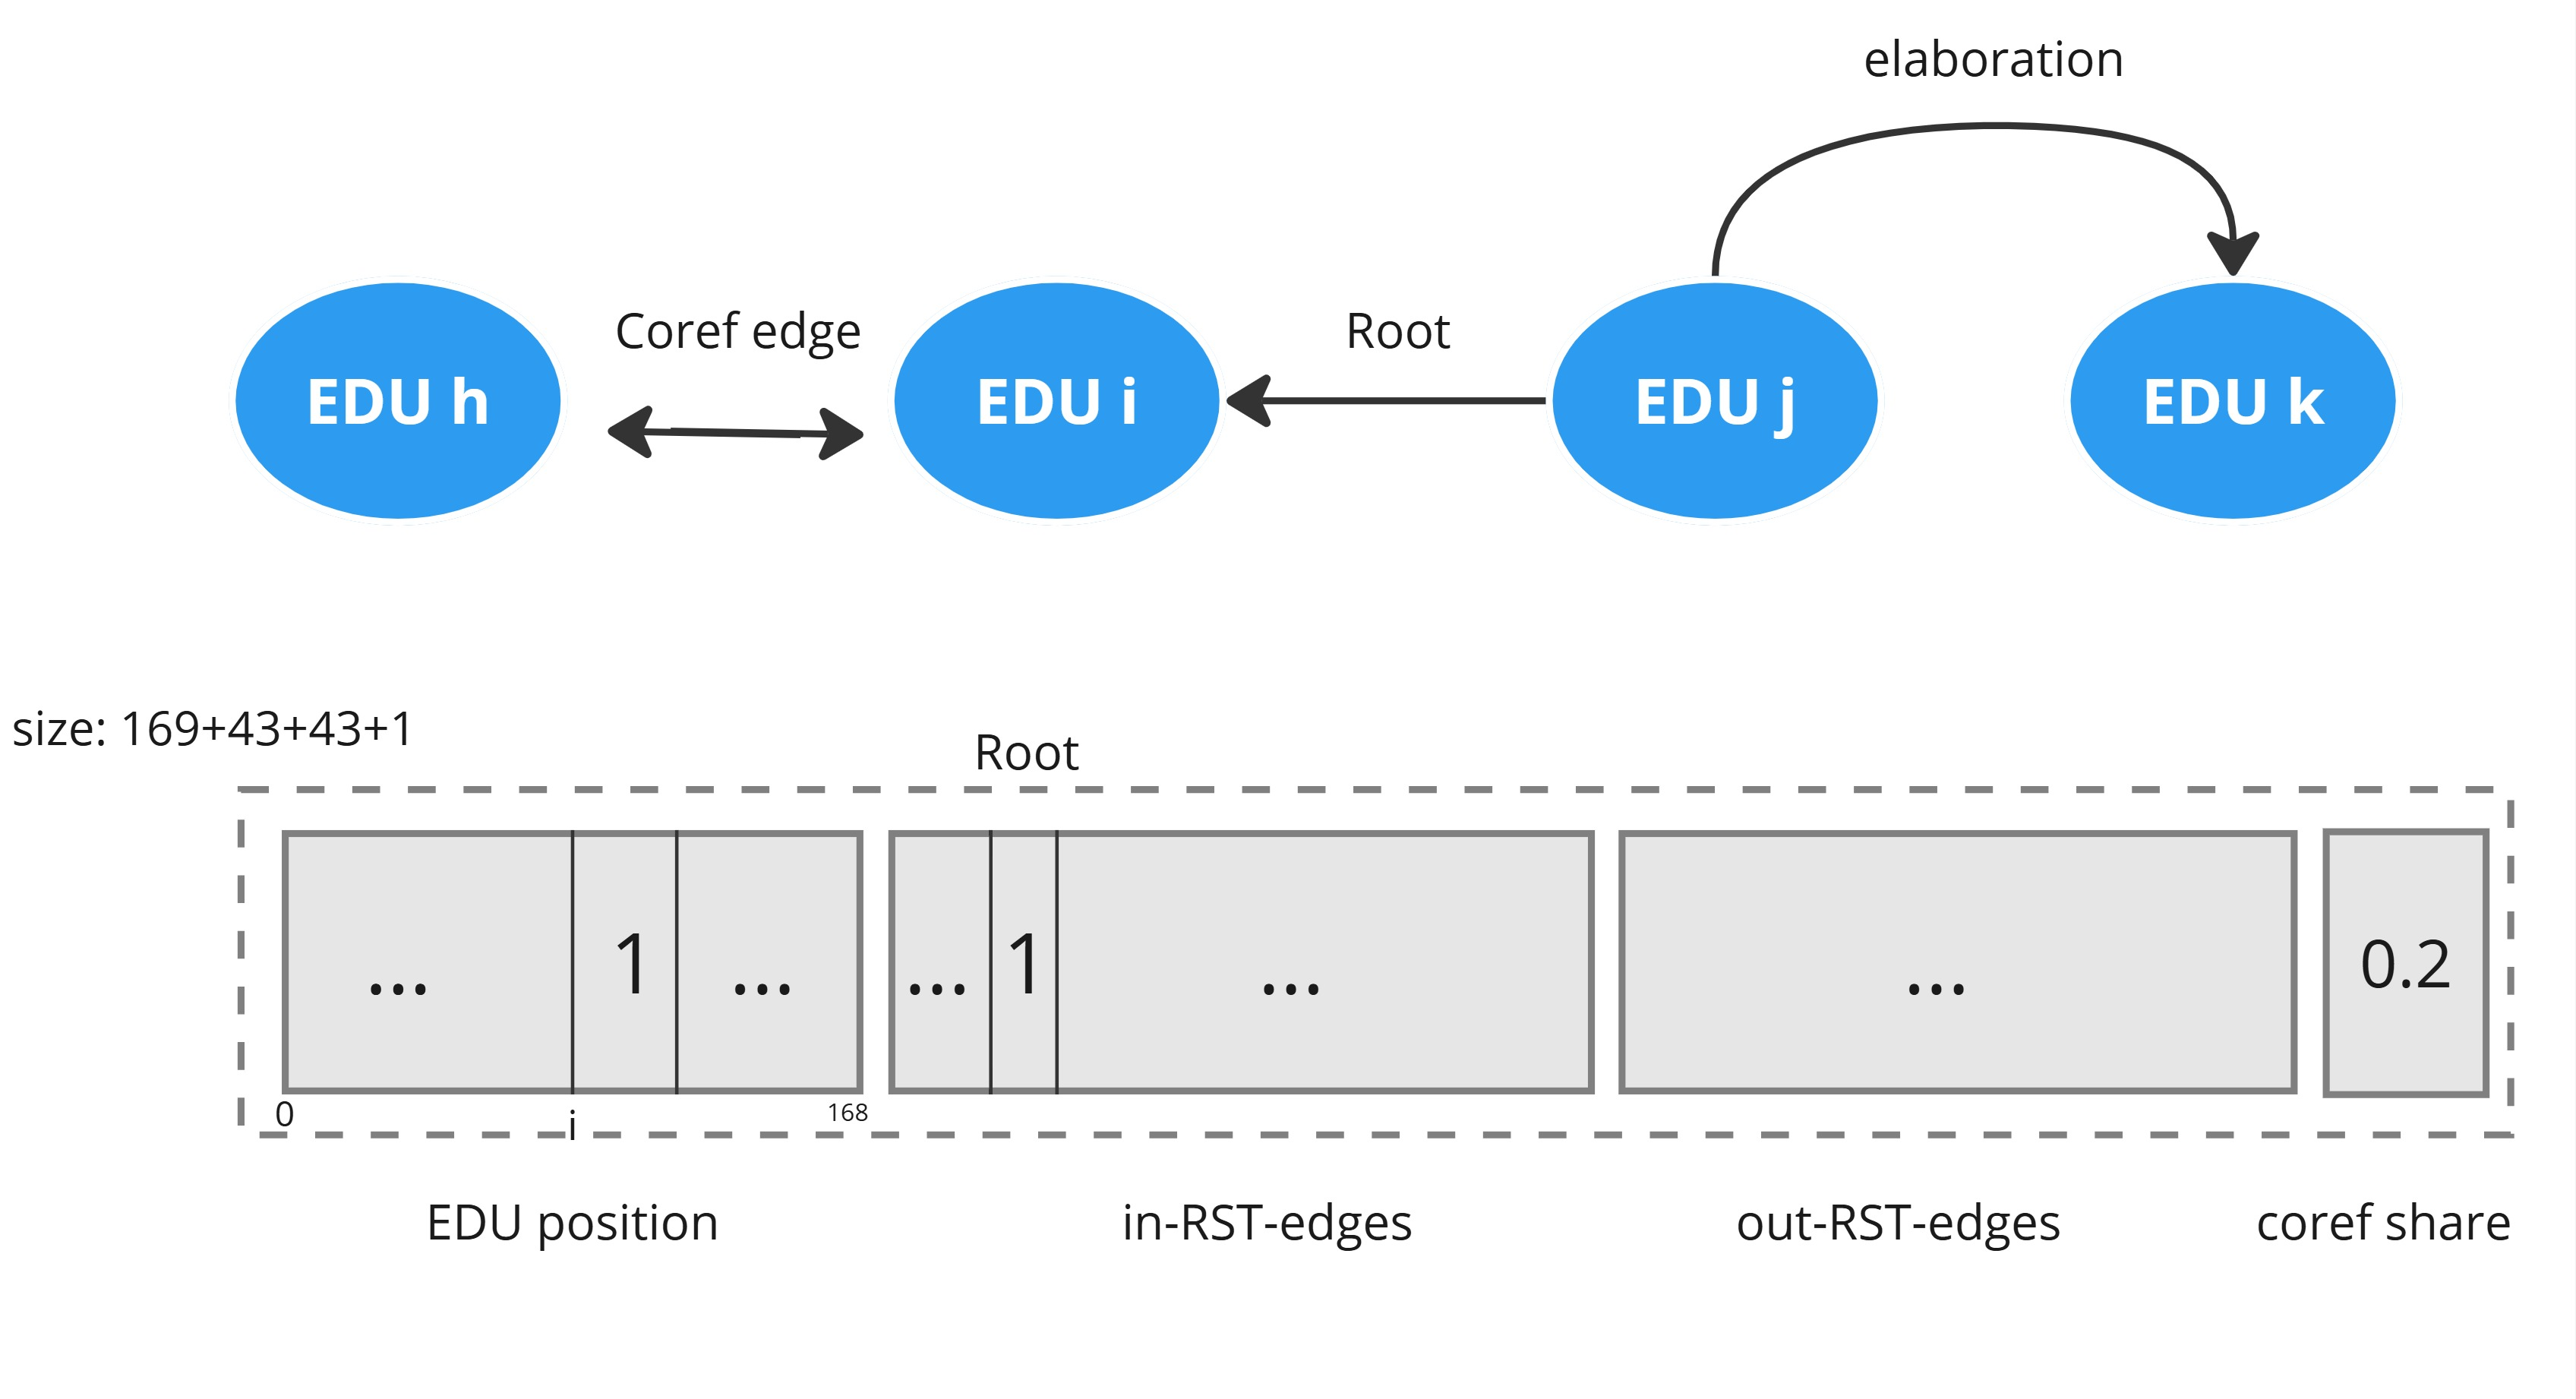
\includegraphics[scale=.05]{imgs/MLP_input_format.jpg}
    \end{minipage}
\end{figure}
\begin{itemize}
    \item As numerically shown in the next four table of results, our MLP performances mainly better than GAT for incorporating graph information
    \item This superiority suggest that not always a complicated architecture outperform its simple alternatives
\end{itemize}

\end{frame}
%---------------------------------------------------------



\section{Results and Discussions}

%---------------------------------------------------------
%Two columns
\begin{frame}
\frametitle{Our 10 Encoder Models on CNNDM}

   \begin{minipage}[t][0.45\textheight][t]{\textwidth}
      \centering
      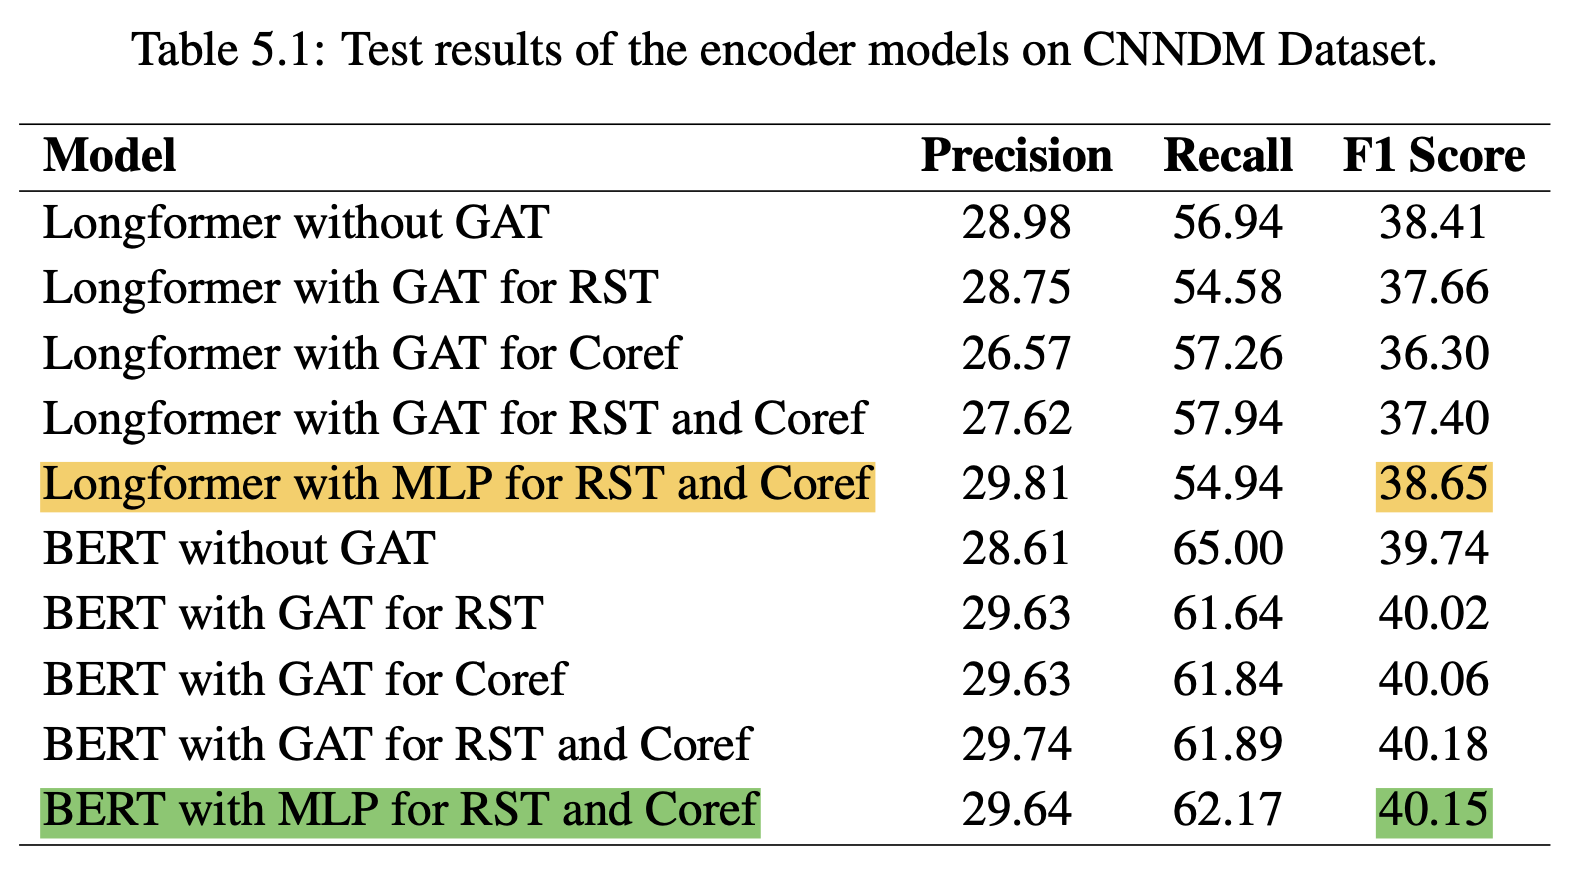
\includegraphics[scale=.33]{imgs/table51_highlight.png}
  \end{minipage}

  % \vfill

  \begin{minipage}[t][0.55\textheight][t]{\textwidth}
    \begin{itemize}
      \item Early versions of "Longformer w.o. GAT" model had $ \approx 35 \% $ F1 score. We used various ML methods to increase it to 38.41\%
      \item Longformer-based models {\tiny \cite{longformer}} have triple the input length of BERT  {\tiny \cite{bert}}, impacting comparisons between these two models.
    \end{itemize}
  \end{minipage}
 
\end{frame}
%---------------------------------------------------------


%---------------------------------------------------------
%Two columns
\begin{frame}
\frametitle{Our 6 Encoder Models on XSum}

   \begin{minipage}[t][0.5\textheight][t]{\textwidth}
      \centering
      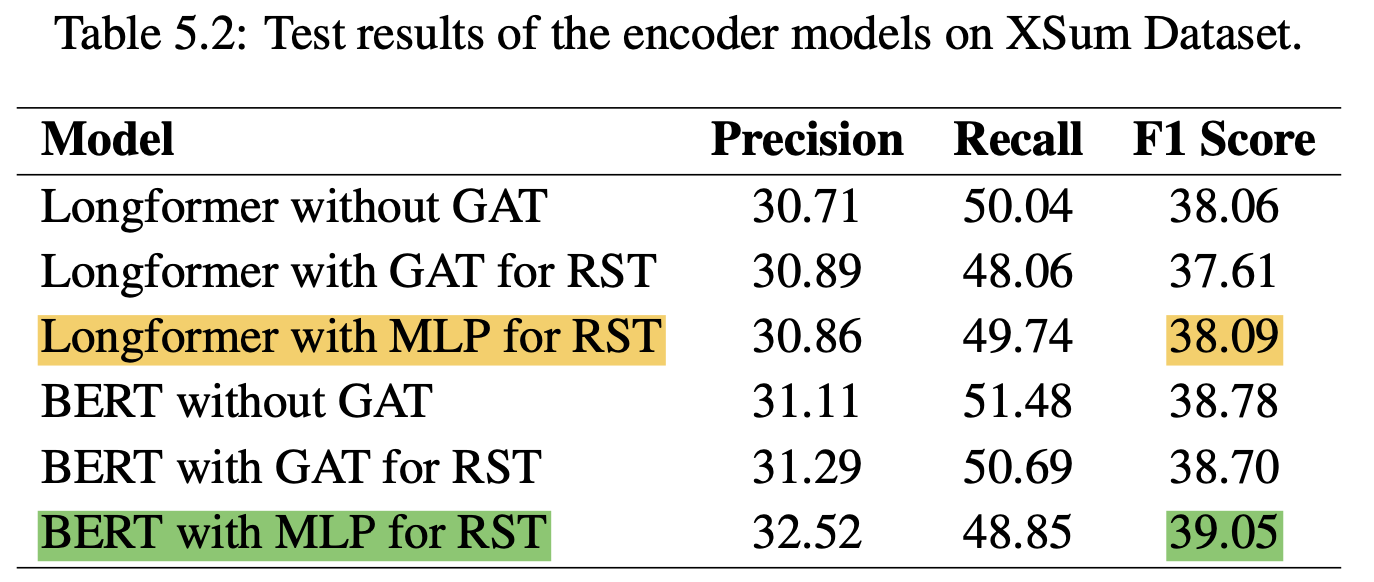
\includegraphics[width=\textwidth]{imgs/table52_highlight.png} 
  \end{minipage}

  \vfill

  \begin{minipage}[t][0.3\textheight][t]{\textwidth}
    \begin{itemize}
      \item MLP-based models show superior performance than their counterparts, showing that incorporating graph information using MLP can help the selection. 
    \end{itemize}
  \end{minipage}
 
\end{frame}
%---------------------------------------------------------

%---------------------------------------------------------
%Two columns
\begin{frame}
\frametitle{Our Decoder Models on CNNDM}

   \begin{minipage}[t][0.5\textheight][t]{\textwidth}
      \centering
      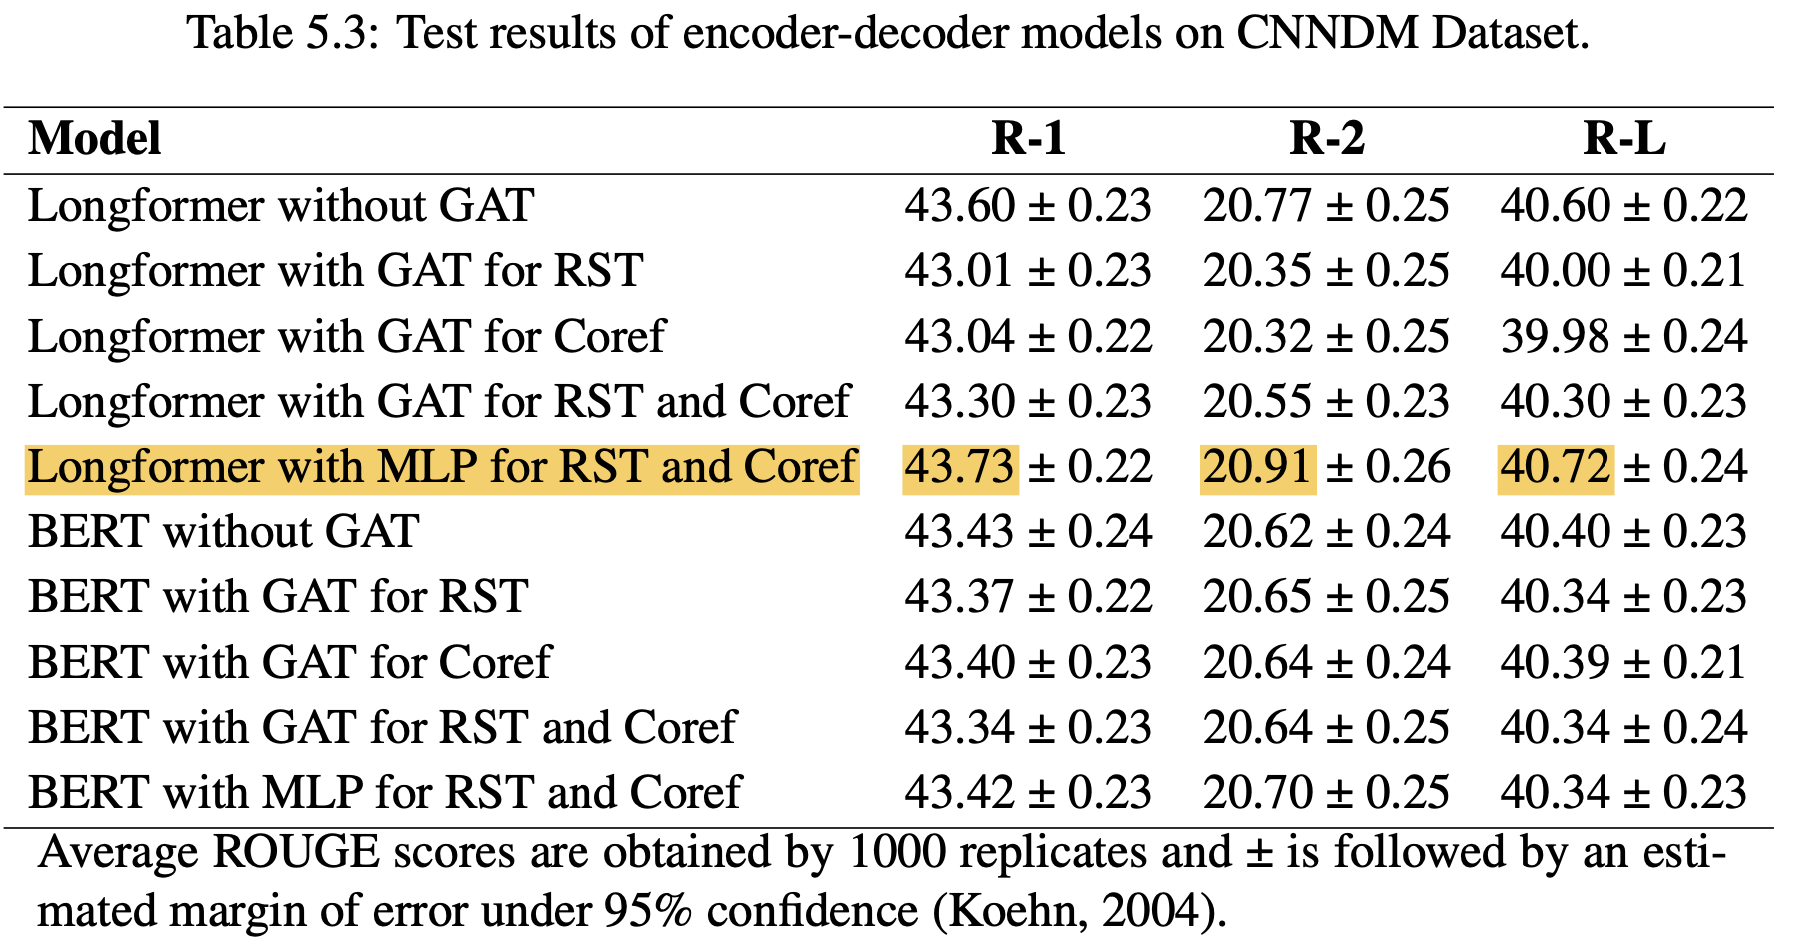
\includegraphics[width=\textwidth]{imgs/table53_highlight.png} 
  \end{minipage}

  \vfill

  \begin{minipage}[t][0.3\textheight][t]{\textwidth}
    \begin{itemize}
      \item Amongst 10 different models, "Longformer with MLP" is performing better, indicating the positive effect of using graph using our MLP approach for long documents.
    \end{itemize}
  \end{minipage}
 
\end{frame}
%---------------------------------------------------------

%---------------------------------------------------------
%Two columns
\begin{frame}
\frametitle{Our Decoder Models on XSum}

   \begin{minipage}[t][0.5\textheight][t]{\textwidth}
      \centering
      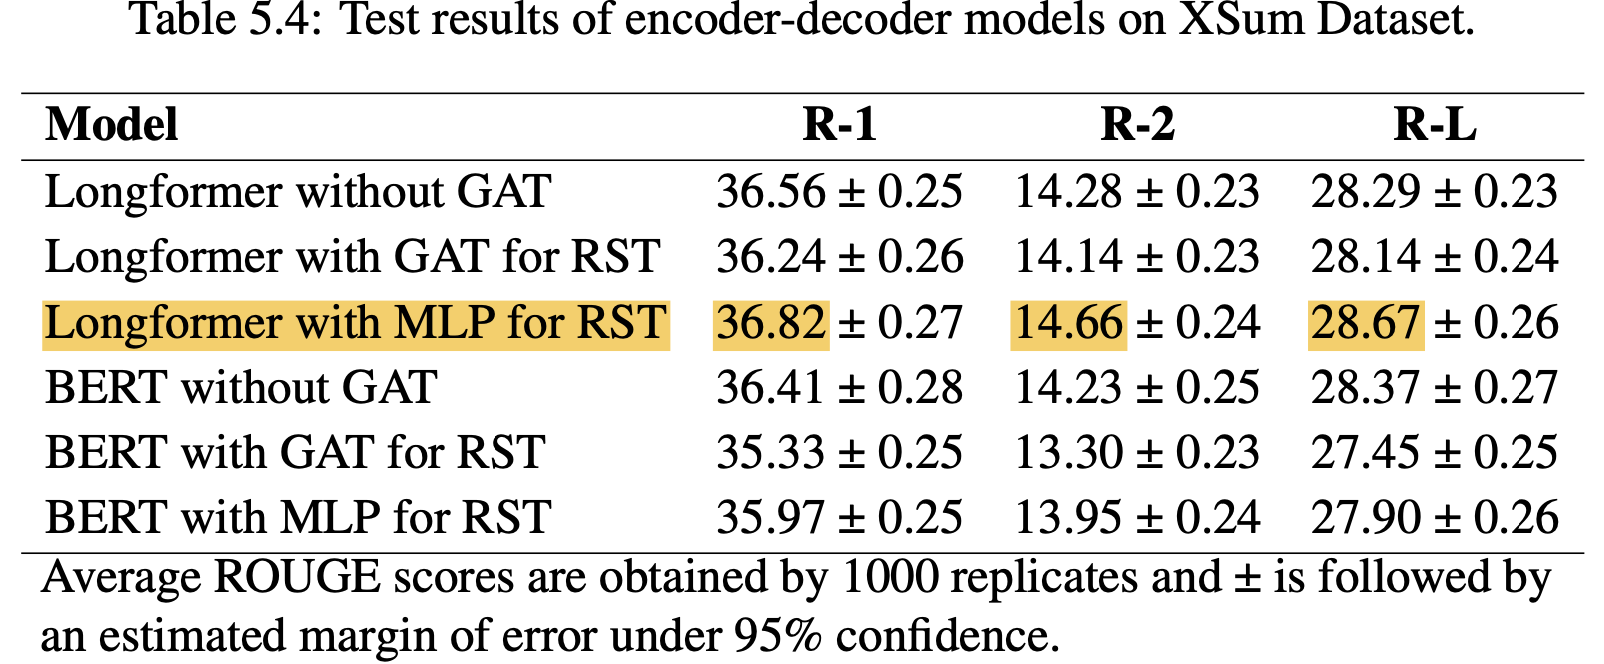
\includegraphics[width=\textwidth]{imgs/table54_highlight.png} 
  \end{minipage}

  \vfill

  \begin{minipage}[t][0.3\textheight][t]{\textwidth}
    \begin{itemize}
      \item Note that we are only using RST graph for XSum, due to time constrants.
    \end{itemize}
  \end{minipage}
 
\end{frame}
%---------------------------------------------------------


%---------------------------------------------------------
%Two columns
\begin{frame}
\frametitle{Outperforming Industry Leaders on CNNDM}

   \begin{minipage}[t][0.5\textheight][t]{\textwidth}
      \centering
      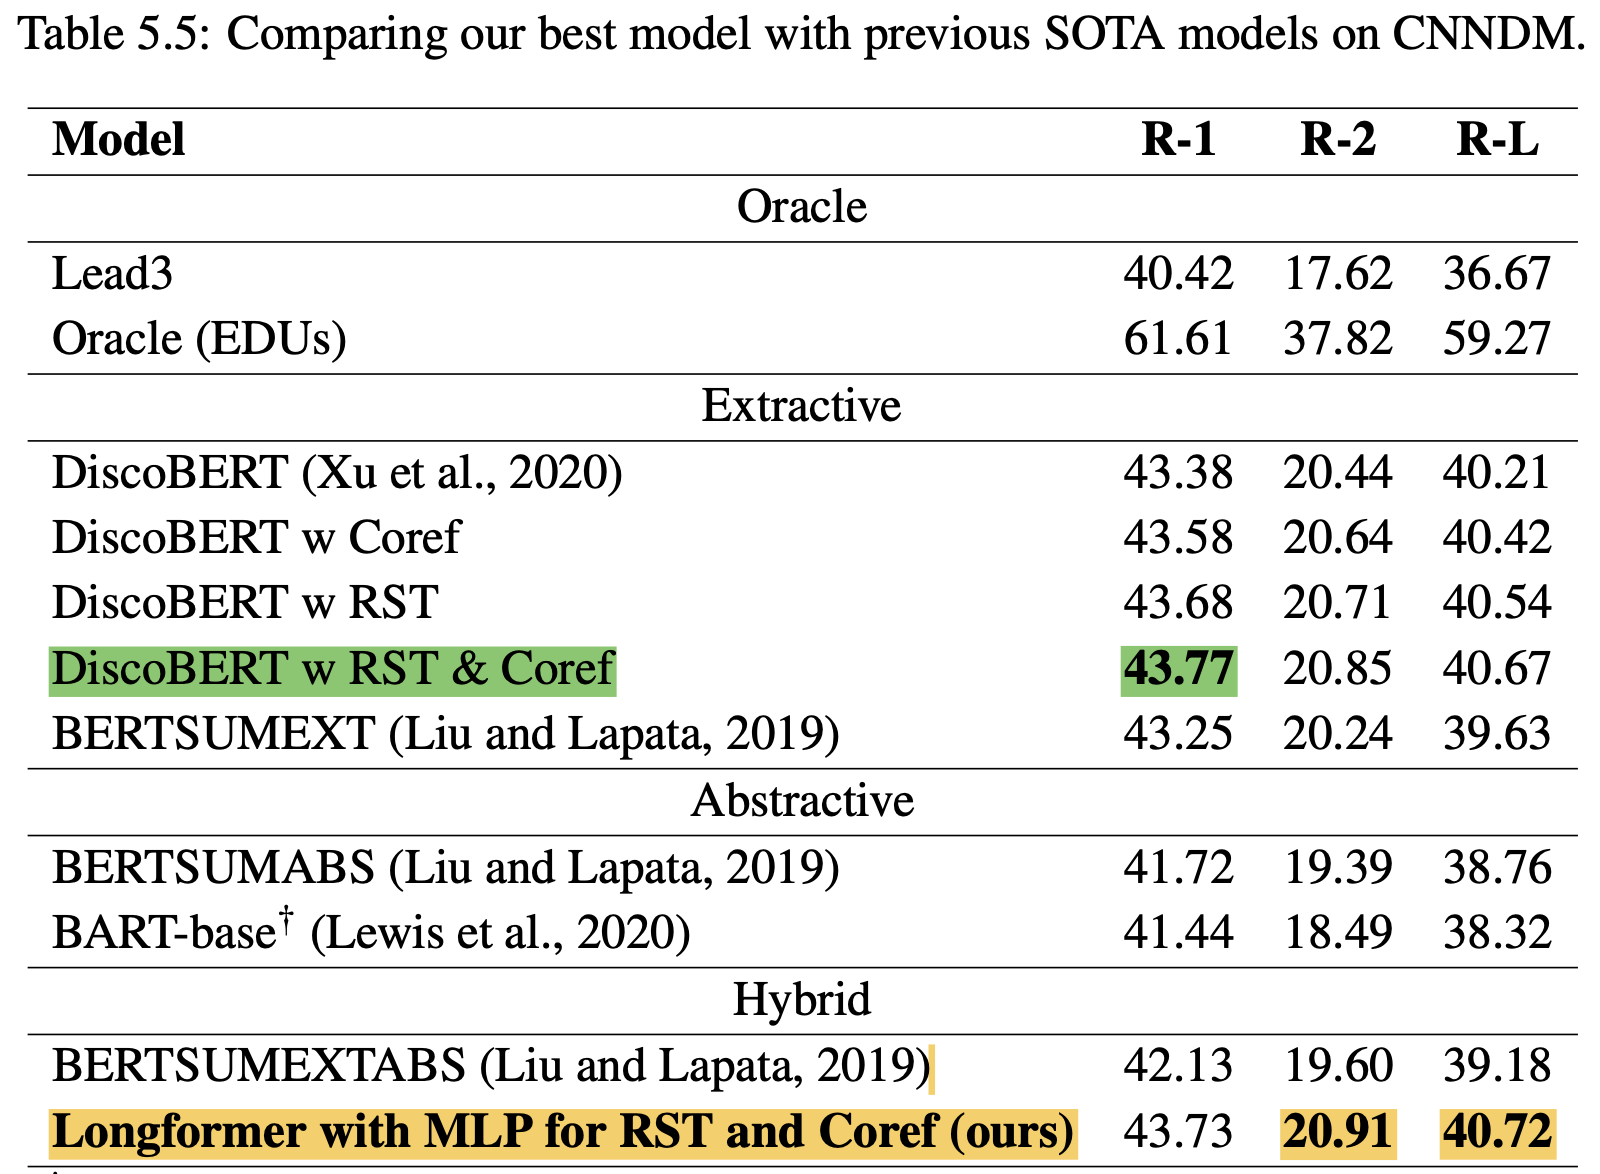
\includegraphics[scale=0.36]{imgs/table55_highlight.png} 
  \end{minipage}
 
\end{frame}
%---------------------------------------------------------


%---------------------------------------------------------
%Two columns
\begin{frame}
\frametitle{Comparison of our Best Model on XSum with Others}

   \begin{minipage}[t][0.5\textheight][t]{\textwidth}
      \centering
      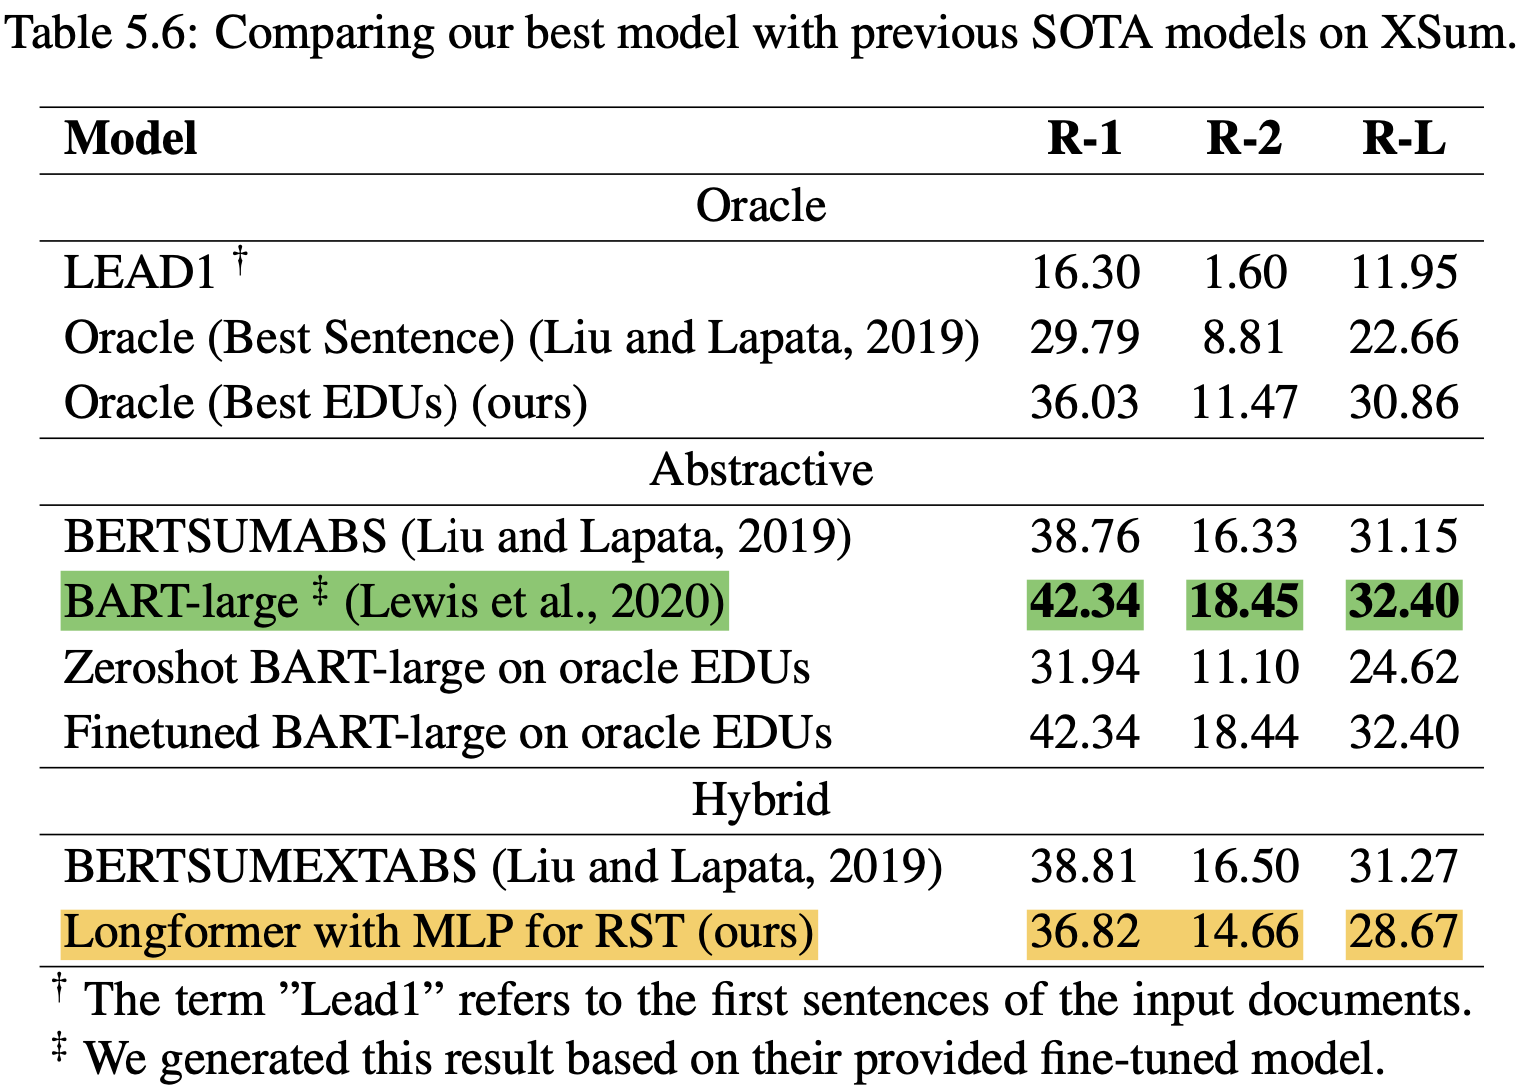
\includegraphics[scale=.3]{imgs/table56_highlight.png} 
  \end{minipage}

  \vfill

  \begin{minipage}[t][0.5\textheight][t]{\textwidth}
    \begin{itemize}
       \item For short documents, using only a decoder might work better.
      \item We used a dataset with the most contrastive characteristics to reveal the limitations of our approach.
    \end{itemize}
  \end{minipage}
 
\end{frame}
%---------------------------------------------------------


%---------------------------------------------------------
%Two columns
\begin{frame}
\frametitle{Effectiveness of Extraction on CNNDM vs XSum}

   \begin{minipage}[t][0.5\textheight][t]{\textwidth}
      \centering
      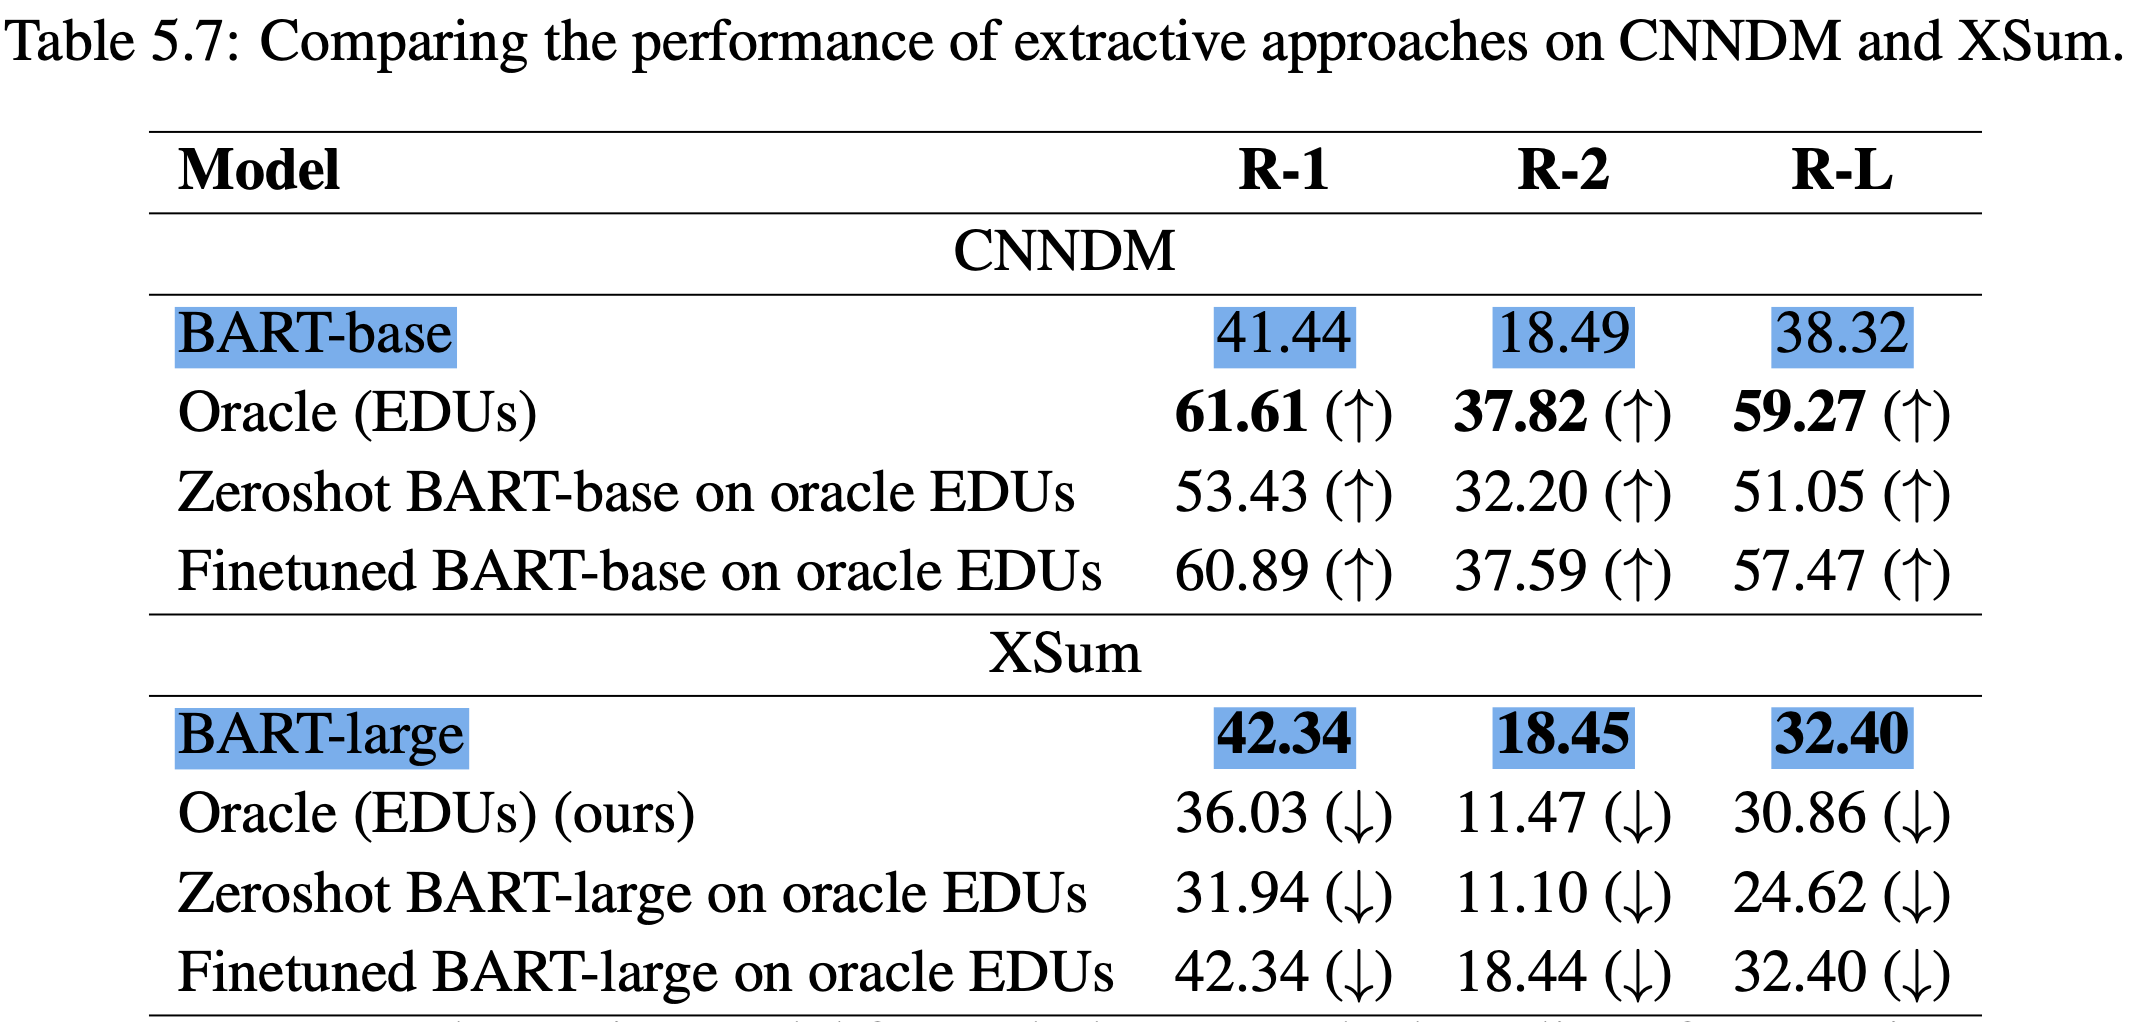
\includegraphics[width=\textwidth]{imgs/table57_highlight.png} 
  \end{minipage}

  \vfill

  \begin{minipage}[t][0.3\textheight][t]{\textwidth}
    \begin{itemize}
      \item Unlike CNNDM dataset, extracting important parts of the XSum dataset does not benefit as much from simply using the entire document as input for the decoder.
    \end{itemize}
  \end{minipage}
 
\end{frame}
%---------------------------------------------------------


\section{Conclusion}


%---------------------------------------------------------
%Highlighting text
\begin{frame}
\frametitle{Conclusion \& Future Directions}

\begin{block}{Outperformed previous SOTA models with simpler graph architecture}
Used a simple MLP rather than a complicated architecture, which outperformed previous SOTA on CNNDM dataset.
\end{block}

\begin{alertblock}{Established a benchmark for graph-based summarization}
Selected a distinctive dataset, annotated it with RST graphs, and established it as a benchmark for future researches.
\end{alertblock}

\begin{exampleblock}{Identified promising future directions}
Looking forward, We recommend using alternative metrics to ROUGE or addressing gradient disconnection by integrating documents and graph information into an end-to-end model.
\end{exampleblock}

\end{frame}
%---------------------------------------------------------


%---------------------------------------------------------
%Highlighting text
\begin{frame}
\frametitle{Q\&A Section}

   \begin{minipage}[t][0.5\textheight][t]{\textwidth}
      \centering
      
\includegraphics[width=\textwidth]{imgs/discuss.jpg} 
  \end{minipage}




\end{frame}
%---------------------------------------------------------

\section{References}

%---------------------------------------------------------
%Highlighting text
\begin{frame}[allowframebreaks]
\frametitle{References}

\vspace*{-\baselineskip}
\setlength{\bibsep}{2pt}
\renewcommand*{\bibfont}{\tiny}
\renewcommand{\refname}{}
\bibliography{mybibfile.bib}

\end{frame}
%---------------------------------------------------------



\end{document}